\documentclass[UTF8,fontset=fandol,11pt,a4paper]{ctexart}
\usepackage[left=23mm,right=23mm,top=23mm,bottom=23mm,headheight=16pt]{geometry}
\usepackage{amsmath,amssymb,bm,mathtools,booktabs,graphicx,array,longtable,adjustbox}
\usepackage{xcolor,fancyhdr,caption,placeins,xurl}
\usepackage[colorlinks=true,linkcolor=blue!40!black,citecolor=blue!40!black,urlcolor=blue!40!black]{hyperref}
\usepackage{bookmark}
\newcommand{\ii}{\mathrm i}
\newcommand{\dd}{\mathrm d}
\newcommand{\Rea}{\operatorname{Re}}
\newcommand{\Ima}{\operatorname{Im}}
\newcommand{\Bin}{B^{\mathrm{inc}}}
\newcommand{\Bref}{B^{\mathrm{ref}}}
\newcommand{\AH}{A_H^{(1)}}
\newcommand{\Aref}{A_{\mathrm{ref}}^{(1)}}
\newcommand{\rp}{r_+}
\newcommand{\rmn}{r_-}
\newcommand{\DeltaK}{\Delta}
\newcommand{\calO}{\mathcal O}
\numberwithin{equation}{section}
\setlength{\parskip}{2pt}
\setlength{\emergencystretch}{3em}
\linespread{1.18}
\allowdisplaybreaks[2]
\raggedbottom
\pagestyle{fancy}\fancyhf{}
\fancyhead[L]{\small Kerr 黑洞的标量场非线性散射}
\fancyhead[R]{\small 解析与数值笔记}
\fancyfoot[C]{\thepage}
\captionsetup{font=small,labelfont=bf}
\renewcommand{\topfraction}{.85}
\renewcommand{\bottomfraction}{.7}
\renewcommand{\textfraction}{.12}
\title{\bfseries Kerr 黑洞的标量场非线性散射\\[3mm]\large 解析推导与数值结果}
\author{}
\date{2026 年 10 月 13 日修订}
\begin{document}
\maketitle
\begin{abstract}
本文整理固定 Kerr 背景上复标量场的弱非线性定态散射理论。从协变场方程出发，推导角向投影、径向 Green 函数和固定入射振幅下的能流修正，说明其与施瓦西径向变量的对应关系。随后用匹配渐近方法求出轴对称三次相互作用的低频吸收系数和复振幅响应，并将单极结果推广至 $|\Phi|^{2n}\Phi$。最后介绍包含物理端点的谱方法及其数值检验，讨论低频幂律、有限频率峰和指数尾的适用范围。数值资料取自稿件 \emph{Infrared hierarchy of nonlinear scalar absorption by Kerr black holes} 的现行本地版本。
\end{abstract}
\tableofcontents
\clearpage

\section{散射问题与弱非线性展开}
\subsection{问题的提出}
黑洞外部的曲率势垒使入射波的一部分被反射，其余部分穿过视界。在线性理论中，给定频率和角模态后，反射率与吸收率不依赖入射振幅。自相互作用改变这一性质：散射系数成为入射强度的函数。本文研究其弱耦合展开的首阶项。

施瓦西和 Kerr 标量波的线性散射已有系统研究\cite{Sanchez1976,Futterman,GlampedakisAndersson2001}。这里沿用相同的入射边界条件，将施瓦西非线性散射的径向 Green 函数方法\cite{HeTianZhangManuscript2026}推广至 Kerr。旋转引入共转视界频率和扁球谐函数，源项因而不能仅由施瓦西有效势替换得到。研究对象为无质量复标量场，背景度规固定，不包含标量能动张量引起的度规反作用。

这一问题与自相互作用标量云\cite{YoshinoKodama2012,Baryakhtar2021,HerdeiroQCloud2014}有共同的局域相互作用，但边界条件不同：标量云研究束缚态或准束缚态，本文讨论无穷远入射的实频率散射。它也不同于引力自力问题\cite{BarackPound2019,PoundWardell2021}，后者包含小天体对场和轨道的反馈。

\subsection{场方程与耦合约定}
采用 $G=c=\hbar=1$ 和度规符号 $(-,+,+,+)$。考虑作用量
\begin{equation}
S=\int\dd^4x\sqrt{-g}\left[-g^{\mu\nu}\partial_\mu\Phi^*\partial_\nu\Phi
+\frac{\epsilon}{2}|\Phi|^4\right].
\end{equation}
对 $\Phi^*$ 变分并分部积分，得到
\begin{equation}\Box\Phi+\epsilon|\Phi|^2\Phi=0.\label{eq:model}\end{equation}
在通常的势能写法 $V=\lambda|\Phi|^4/2$ 下，$\epsilon=-\lambda$。以下所有首阶系数均按式\eqref{eq:model}定义；耦合符号决定实际能流修正的方向。

令
\begin{equation}
\Phi=\Phi^{(0)}+\epsilon\Phi^{(1)}+\calO(\epsilon^2).
\end{equation}
比较同阶项得
\begin{align}
\Box\Phi^{(0)}&=0,\label{eq:zero}\\
\Box\Phi^{(1)}&=-|\Phi^{(0)}|^2\Phi^{(0)}.\label{eq:first}
\end{align}
因此首阶计算分为齐次散射问题和由零阶场产生的有源问题。若零阶场的时间、方位角依赖为 $e^{-\ii\omega t+\ii m\phi}$，则源具有相同的依赖：
\begin{equation}
|e^{-\ii\omega t+\ii m\phi}|^2e^{-\ii\omega t+\ii m\phi}=e^{-\ii\omega t+\ii m\phi}.
\end{equation}
频率和 $m$ 不变，而角函数的乘积一般激发多个 $\ell$。单频闭合依赖复场及其 $U(1)$ 对称相互作用；实场的三次源还会产生 $3\omega$ 等谐波。

按 $[\Phi]=M^{-1}$，$\epsilon$ 无量纲。扰动近似要求相互作用在所考察区域足够弱，例如
\begin{equation}
|\epsilon|M^2\max_{\mathcal D}|\Phi^{(0)}|^2\ll1.
\end{equation}
散射振幅的首阶相对变化也须小于一，其表达式将在第\ref{sec:nonlinear}节给出。

\subsection{施瓦西径向约化}
施瓦西度规和龟坐标满足
\begin{equation}
\dd s^2=-f\dd t^2+f^{-1}\dd r^2+r^2\dd\Omega^2,
\qquad f=1-\frac{2M}{r},\qquad \frac{\dd r_*}{\dd r}=f^{-1}.
\end{equation}
取 $\Phi=e^{-\ii\omega t}Y_{\ell m}u(r)/r$，其中 $\int|Y_{\ell m}|^2\dd\Omega=1$。波算符给出
\begin{equation}
\Box\Phi=\frac{e^{-\ii\omega t}Y_{\ell m}}{rf}
\left[\frac{\dd^2u}{\dd r_*^2}+(\omega^2-V_\ell)u\right],
\qquad V_\ell=f\left[\frac{\ell(\ell+1)}{r^2}+\frac{2M}{r^3}\right].
\end{equation}
由式\eqref{eq:first}，自通道的首阶径向方程为
\begin{equation}
\frac{\dd^2u_1}{\dd r_*^2}+(\omega^2-V_\ell)u_1
=-\frac{f}{r^2}\mathcal C_\ell|u_0|^2u_0,
\qquad \mathcal C_\ell=\int|Y_{\ell m}|^4\dd\Omega.
\end{equation}
源的 $f/r^2$ 权重由协变方程和 $1/r$ 场重定义共同产生。视界处 $u_0\sim e^{-\ii\omega r_*}$，无穷远处
\begin{equation}
u_0\sim\widehat I e^{-\ii\omega r_*}+\widehat R e^{\ii\omega r_*}.
\end{equation}
Kerr 中采用未约化径向函数 $R$，无穷远渐近行为自带 $1/r$。两种变量的换算将在能流修正之后讨论。

\section{Kerr 上的线性标量散射}
\label{sec:linear}
\subsection{几何与变量分离}
定义
\begin{align}
\Sigma&=r^2+a^2\cos^2\theta,&\Delta&=r^2-2Mr+a^2=(r-r_+)(r-r_-),\\
r_\pm&=M\pm\sqrt{M^2-a^2},&H&=r^2+a^2.
\end{align}
在 Boyer--Lindquist 坐标中，Kerr 度规为
\begin{align}
\dd s^2={}&-\left(1-\frac{2Mr}{\Sigma}\right)\dd t^2
-\frac{4Mar\sin^2\theta}{\Sigma}\dd t\dd\phi
+\frac{\Sigma}{\Delta}\dd r^2+\Sigma\dd\theta^2\nonumber\\
&+\frac{H^2-a^2\Delta\sin^2\theta}{\Sigma}\sin^2\theta\dd\phi^2.
\end{align}
视界角速度、表面引力和龟坐标满足
\begin{equation}
\Omega_H=\frac{a}{r_+^2+a^2},\qquad
\kappa=\frac{r_+-r_-}{2(r_+^2+a^2)},\qquad
\frac{\dd r_*}{\dd r}=\frac H\Delta.
\end{equation}
对亚极端黑洞，龟坐标可取
\begin{equation}
r_*=r+\frac{2Mr_+}{r_+-r_-}\ln\frac{r-r_+}{2M}
-\frac{2Mr_-}{r_+-r_-}\ln\frac{r-r_-}{2M}+C.
\end{equation}
常数 $C$ 改变渐近振幅的相位，不改变一致归一化下的能流。

由于 $\sqrt{-g}=\Sigma\sin\theta$，标量波算符可写为
\begin{align}
\Sigma\Box={}&\partial_r(\Delta\partial_r)
+\frac1{\sin\theta}\partial_\theta(\sin\theta\partial_\theta)
-\left(\frac{H^2}{\Delta}-a^2\sin^2\theta\right)\partial_t^2\nonumber\\
&-\frac{4Mar}{\Delta}\partial_t\partial_\phi
+\left(\frac1{\sin^2\theta}-\frac{a^2}{\Delta}\right)\partial_\phi^2.
\end{align}
令
\begin{equation}
\Phi^{(0)}=e^{-\ii\omega t+\ii m\phi}S_{\ell m}(\theta;a\omega)R_{\ell m\omega}(r),
\quad\int\dd\Omega\,|S_{\ell m}|^2=1.
\end{equation}
代入式\eqref{eq:zero}，利用 $H-\Delta=2Mr$ 整理混合项，得到角方程
\begin{equation}
\left[\frac1{\sin\theta}\frac\dd{\dd\theta}\left(\sin\theta\frac\dd{\dd\theta}\right)
+a^2\omega^2\cos^2\theta-\frac{m^2}{\sin^2\theta}+A_{\ell m}\right]S_{\ell m}=0
\end{equation}
和 $s=0$ 的 Teukolsky 径向方程\cite{Teukolsky1973}
\begin{align}
\mathcal LR&\equiv(\Delta R')'+VR=0,\label{eq:radial}\\
V&=\frac{K^2}{\Delta}-\lambda,\qquad
K=\omega H-am,\qquad \lambda=A_{\ell m}+a^2\omega^2-2am\omega.
\end{align}
以下撇号均表示 $r$ 导数。$A_{\ell m}$ 是角本征值，$\lambda$ 是径向分离常数，两者在 Kerr 上一般不同。
当 $a\omega\to0$ 时，$S_{\ell m}e^{\ii m\phi}\to Y_{\ell m}$，$A_{\ell m}\to\ell(\ell+1)$。

\subsection{散射边界条件}
视界生成元为 $\partial_t+\Omega_H\partial_\phi$，因此视界相位由
\begin{equation}p=\omega-m\Omega_H\end{equation}
决定。归一化为单位视界入射振幅的解 $R_{\rm in}$ 满足
\begin{align}
R_{\rm in}&\sim e^{-\ii p r_*},&&r\to r_+,\label{eq:bcH}\\
R_{\rm in}&\sim\frac{\Bin e^{-\ii\omega r_*}+\Bref e^{\ii\omega r_*}}r,
&&r\to\infty.\label{eq:bcInf}
\end{align}
另取两支在无穷远归一化的解
\begin{equation}
R_{\rm down}\sim\frac{e^{-\ii\omega r_*}}r,\qquad
R_{\rm up}\sim\frac{e^{\ii\omega r_*}}r.
\end{equation}
$R_{\rm in}$ 在未来视界正则，$R_{\rm up}$ 用于构造无穷远出射 Green 函数。这一散射归一化也用于 Teukolsky 解析解的振幅定义\cite{MST1996}。

\subsection{径向守恒流与吸收系数}
定义径向流
\begin{equation}
J[R]=\frac{\Delta}{2\ii}(R^*R'-RR'^*)=\Delta\Ima(R^*R').
\end{equation}
式\eqref{eq:radial}在实频率下系数为实数，故
\begin{equation}J'=\Ima[R^*(\Delta R')']=\Ima(-V|R|^2)=0.\end{equation}
与之对应的能量通量来自应力张量
\begin{equation}
T_{\mu\nu}=\partial_\mu\Phi^*\partial_\nu\Phi+\partial_\nu\Phi^*\partial_\mu\Phi
+g_{\mu\nu}\left[-\partial_\alpha\Phi^*\partial^\alpha\Phi+\frac\epsilon2|\Phi|^4\right].
\end{equation}
对于时间 Killing 场，$j_E^\mu=-T^\mu{}_t$。相互作用势不贡献径向混合分量，因为 $\delta^r{}_t=0$。单模态给出
\begin{equation}
T^r{}_t=-\frac{2\omega\Delta}{\Sigma}|S|^2\Ima(R^*R'),\qquad
\mathcal F_{\rm out}=\int\sqrt{-g}\,j_E^r\dd\theta\dd\phi=2\omega J.
\end{equation}
代入边界条件，得到
\begin{align}
J_\infty&=\omega(|\Bref|^2-|\Bin|^2),&J_H&=-p(r_+^2+a^2),\\
\mathcal F_{\rm inc}&=2\omega^2|\Bin|^2,&\mathcal F_{\rm ref}&=2\omega^2|\Bref|^2,\\
\mathcal F_H&=2\omega p(r_+^2+a^2).
\end{align}
这里 $\mathcal F_H$ 以流入视界为正。除以入射通量便得
\begin{equation}
T^{(0)}=\frac{p(r_+^2+a^2)}{\omega|\Bin|^2},\qquad
R^{(0)}=\frac{|\Bref|^2}{|\Bin|^2},\qquad T^{(0)}+R^{(0)}=1.\label{eq:T0}
\end{equation}
$p<0$ 时视界吸收负的 Killing 能量，$T^{(0)}<0$、$R^{(0)}>1$，即超辐射。
本文主要数值结果取 $m=0$，此时 $p=\omega$，$T^{(0)}$ 为非负吸收率。

\section{首阶非线性散射与能流修正}
\label{sec:nonlinear}
\subsection{角投影与有源径向方程}
以一个 $(\ell,m,\omega)$ 模态作为零阶入射场，展开
\begin{equation}
\Phi^{(1)}=e^{-\ii\omega t+\ii m\phi}\sum_{\ell'}S_{\ell'm}R^{(1)}_{\ell'|\ell m\omega}.
\end{equation}
分离式\eqref{eq:first}时需要先乘以 $\Sigma$。以 $S_{\ell'm}^*$ 作角投影，得到
\begin{align}
\mathcal L_{\ell'm\omega}R^{(1)}_{\ell'|\ell m\omega}&=-Q_{\ell'\ell m},\\
Q_{\ell'\ell m}&=(r^2C^{(0)}_{\ell'\ell m}+a^2C^{(2)}_{\ell'\ell m})|R_0|^2R_0,\label{eq:source}\\
C^{(j)}_{\ell'\ell m}&=\int\dd\Omega\,\cos^j\theta\,S_{\ell'm}^*|S_{\ell m}|^2S_{\ell m},\quad j=0,2.
\end{align}
两个径向权重分别来自 $\Sigma$ 的 $r^2$ 与 $a^2\cos^2\theta$ 部分。对自通道 $\ell'=\ell$，投影系数均为实数。
扁球谐函数的正交性使 $\ell'\ne\ell$ 的首阶场与零阶场在角积分后不发生干涉；这些通道的独立能流始于 $\epsilon^2$。所以计算总能流的一阶修正只需自通道，但完整的一阶场仍具有角模式耦合。

\subsection{Green 函数及边界振幅}
在指定目标通道中取 $R_{\rm in},R_{\rm up}$，定义
\begin{equation}
W=\Delta(R_{\rm in}R_{\rm up}'-R_{\rm up}R_{\rm in}').
\end{equation}
两支齐次解的方程给出 $W'=0$。由此构造
\begin{equation}
G(r,r')=\frac{R_{\rm in}(r_<)R_{\rm up}(r_>)}W.
\end{equation}
它在 $r=r'$ 连续，并满足
\begin{equation}
\Delta(r')[\partial_rG|_{r=r'+0}-\partial_rG|_{r=r'-0}]=1,
\end{equation}
故 $\mathcal LG=\delta(r-r')$。对于 $\mathcal LR_1=-Q$，
\begin{align}
R_1(r)&=-\frac{R_{\rm up}(r)I_{\rm in}(r)+R_{\rm in}(r)I_{\rm up}(r)}W,\label{eq:R1green}\\
I_{\rm in}(r)&=\int_{r_+}^{r}R_{\rm in}(s)Q(s)\dd s,\\
I_{\rm up}(r)&=\int_{r}^{\infty}R_{\rm up}(s)Q(s)\dd s.
\end{align}
一阶解在视界纯入射，在无穷远纯出射，不改变给定的入射波。两端渐近系数为
\begin{equation}
\AH=-\frac1W\int_{r_+}^\infty R_{\rm up}Q\dd r,\qquad
\Aref=-\frac1W\int_{r_+}^\infty R_{\rm in}Q\dd r.\label{eq:amplitudes}
\end{equation}
同一归一化必须同时用于齐次解、Wronskian 和源。式\eqref{eq:amplitudes}按单位视界零阶振幅定义，尚不是单位入射场的首阶振幅。

\subsection{固定入射振幅}
在 $R_0\mapsto\alpha R_0$ 下，三次源及首阶场按 $|\alpha|^2\alpha$ 缩放。
取 $\alpha=1/\Bin$，单位入射场的视界和反射振幅为
\begin{align}
H_{\rm fix}&=\frac1{\Bin}+\epsilon\frac{\AH}{|\Bin|^2\Bin},\\
\mathcal R_{\rm fix}&=\frac{\Bref}{\Bin}+\epsilon\frac{\Aref}{|\Bin|^2\Bin}.
\end{align}
使用 $|x+\epsilon y|^2=|x|^2+2\epsilon\Rea(x^*y)+\calO(\epsilon^2)$，能流展开为
\begin{align}
T^{(1)}&=\frac{2p(r_+^2+a^2)}{\omega|\Bin|^4}\Rea\AH,\label{eq:T1}\\
R^{(1)}&=\frac{2\Rea(\overline{\Bref}\Aref)}{|\Bin|^4}.\label{eq:Ref1}
\end{align}
若指定入射振幅为无量纲 $\mathcal A_{\rm in}$，则
\begin{align}
T&=T^{(0)}+\epsilon|\mathcal A_{\rm in}|^2T^{(1)}+\calO(\epsilon^2|\mathcal A_{\rm in}|^4),\\
R&=R^{(0)}+\epsilon|\mathcal A_{\rm in}|^2R^{(1)}+\calO(\epsilon^2|\mathcal A_{\rm in}|^4).
\end{align}
定义相对复振幅和相对吸收响应
\begin{equation}
\rho_H=\frac{\AH}{|\Bin|^2},\qquad
\chi_H=2\Rea\rho_H=\frac{T^{(1)}}{T^{(0)}}\quad(p\ne0).\label{eq:rho}
\end{equation}
首阶视界相位变化为
\begin{equation}\delta\arg H=\epsilon|\mathcal A_{\rm in}|^2\Ima\rho_H+\calO(\epsilon^2).\end{equation}
因此实部决定吸收变化，虚部决定相位变化。边界振幅的扰动条件是
$|\epsilon||\mathcal A_{\rm in}|^2|\rho_H|\ll1$，而不仅是吸收的实部修正小。
在 $p=0$ 处，式\eqref{eq:rho}用 $2\Rea\rho_H$ 定义而不作 $0/0$ 比值。
若振幅在阈值附近平滑，$T^{(0)}=p\tau_0+\cdots$、$T^{(1)}=p\tau_1+\cdots$，两者同时消失并不导致相对响应发散。

\subsection{首阶能流守恒}
将径向流展开到首阶，交叉项为
\begin{equation}
J_1=\Delta\Ima(R_0^*R_1'+R_1^*R_0').
\end{equation}
由零阶和首阶方程可得
\begin{equation}J_1'=-\Ima(R_0^*Q)=0,\end{equation}
因为自通道的 $Q$ 为实权重乘以 $|R_0|^2R_0$。
两端流相等且一阶无额外入射波，故
\begin{equation}T^{(1)}+R^{(1)}=0.\label{eq:balance1}\end{equation}
局域相互作用重新分配吸收与反射能量，而不构成外部能量源。这一恒等式也是数值检验，但不能排除两端具有共同误差。

\subsection{施瓦西归一化的对应}
在 $a=0$ 下，若施瓦西约化解 $u$ 的视界振幅为一，则单位视界 Teukolsky 解为
\begin{equation}
R_{\rm in}=\frac{r_+u}{r},\qquad \Bin=r_+\widehat I,\qquad\Bref=r_+\widehat R.
\end{equation}
同一源符号下，三次齐次性给出
\begin{equation}
\AH=r_+^2\widehat A_H^{(1)},\qquad\Aref=r_+^3\widehat A_{\rm ref}^{(1)}.
\end{equation}
代入式\eqref{eq:T1}--\eqref{eq:Ref1}，得到
\begin{equation}
T^{(1)}_{\rm unit-inc}=\frac{2\Rea\widehat A_H^{(1)}}{|\widehat I|^4},\qquad
R^{(1)}_{\rm unit-inc}=\frac{2\Rea(\widehat R^*\widehat A_{\rm ref}^{(1)})}{|\widehat I|^4}.
\end{equation}
若旧约定的首阶系数分母为 $|\widehat I|^2$，则
\begin{equation}
T^{(1)}_{\rm unit-inc}=T^{(0)}\widehat T^{(1)},\qquad
R^{(1)}_{\rm unit-inc}=T^{(0)}\widehat R^{(1)}.
\end{equation}
参考施瓦西稿件\cite{HeTianZhangManuscript2026}写作
$\Box\phi=\lambda_{\rm ref}|\phi|^{2N-2}\phi$，故还须作 $N=n+1$、$\epsilon_n=-\lambda_{\rm ref}$ 的换算。
物理能流不依赖径向变量的选择，但按不同耦合与归一化定义的首阶系数不能直接比较。

\section{低频渐近理论}
\label{sec:IR}
\subsection{轴对称静态解与远区匹配}
固定 $|a|<M$，取 $m=0$，令 $\omega\to0$。近区 $r\ll\omega^{-1}$ 和远区 $r\gg M$ 的重叠区域为
$M\ll r\ll\omega^{-1}$。静态角本征值为 $\ell(\ell+1)$，径向方程化为
\begin{equation}(\Delta R')'-\ell(\ell+1)R=0.\end{equation}
令 $d=\sqrt{M^2-a^2}$、$\xi=(r-M)/d$，则 $\Delta=d^2(\xi^2-1)$，方程成为
\begin{equation}
\frac\dd{\dd\xi}\left[(\xi^2-1)\frac{\dd R}{\dd\xi}\right]-\ell(\ell+1)R=0.
\end{equation}
视界正则、单位归一化的解为 $R=P_\ell(\xi)$。其大 $\xi$ 首项为
\begin{equation}
P_\ell(\xi)\sim q_\ell\xi^\ell,\qquad q_\ell=\frac{(2\ell)!}{2^\ell(\ell!)^2}.
\end{equation}
远区以 $x=\omega r$ 为变量，领先方程为
\begin{equation}
\frac\dd{\dd x}\left(x^2\frac{\dd R}{\dd x}\right)
+[x^2-\ell(\ell+1)]R=0.
\end{equation}
在重叠区 $j_\ell(x)\sim x^\ell/(2\ell+1)!!$，因此
\begin{align}
R_{\rm in}&=\mathcal K_\ell(M\omega)^{-\ell}j_\ell(x)[1+o(1)],\\
\mathcal K_\ell&=(2\ell+1)!!\,q_\ell(M/d)^\ell.\label{eq:Kmatch}
\end{align}
利用 $j_\ell(x)\sim\sin(x-\ell\pi/2)/x$，读出入射振幅及线性吸收：
\begin{align}
\Bin&=\frac{M\ii^{\ell+1}\mathcal K_\ell}{2(M\omega)^{\ell+1}}[1+o(1)],\label{eq:BIR}\\
T^{(0)}_{\ell0}&=\mathcal A_\ell^{(0)}(M\omega)^{2\ell+2}[1+o(1)],\label{eq:T0IR}\\
\mathcal A_\ell^{(0)}&=\frac{4(r_+^2+a^2)}{M^2\mathcal K_\ell^2}.
\end{align}
角势垒决定指数 $2\ell+2$，视界几何和近区匹配决定系数。

\subsection{三次相互作用的复响应}
在远区，协变源式\eqref{eq:source}的领先项为 $r^2\mathcal C_\ell R_{\rm in}^3$，其中
\begin{equation}\mathcal C_\ell=\int|Y_{\ell0}|^4\dd\Omega.\end{equation}
固定自旋的强场区域与 $a^2C^{(2)}$ 权重贡献次领先项。为计算领先 Green 积分，暂设 $M=1$，取
\begin{equation}
R_{\rm up}=\omega\ii^{\ell+1}h_\ell^{(1)}(x)[1+o(1)],\quad
W=2\ii\omega\Bin=\ii^{\ell+2}\mathcal K_\ell\omega^{-\ell}[1+o(1)].
\end{equation}
$h_\ell^{(1)}=j_\ell+\ii y_\ell$，其相位使 $R_{\rm up}$ 在无穷远的出射振幅为一。
将 $r^2\dd r=x^2\dd x/\omega^3$ 代入式\eqref{eq:amplitudes}，有
\begin{equation}
\AH=\ii\mathcal C_\ell\mathcal K_\ell^2\omega^{-2\ell-2}
\int_0^\infty x^2 h_\ell^{(1)}(x)j_\ell^3(x)\dd x\,[1+o(1)].
\end{equation}
定义收敛的积分
\begin{align}
\mathcal I_\ell&=-\int_0^\infty x^2y_\ell(x)j_\ell^3(x)\dd x,\\
\mathcal J_\ell&=\int_0^\infty x^2j_\ell^4(x)\dd x>0.
\end{align}
因 $\ii h_\ell^{(1)}=-y_\ell+\ii j_\ell$，恢复 $M$ 后得
\begin{equation}
\frac{\AH}{M^2}=\mathcal C_\ell\mathcal K_\ell^2
(\mathcal I_\ell+\ii\mathcal J_\ell)(M\omega)^{-2\ell-2}[1+o(1)].\label{eq:AHIR}
\end{equation}
式\eqref{eq:AHIR}与式\eqref{eq:BIR}组合，近区匹配系数消去：
\begin{align}
\rho_{H,\ell0}&\longrightarrow4\mathcal C_\ell(\mathcal I_\ell+\ii\mathcal J_\ell),\label{eq:rhoIR}\\
\chi_{H,\ell0}&\longrightarrow\chi_\ell^{\rm IR}=8\mathcal C_\ell\mathcal I_\ell,\\
T^{(1)}_{\ell0}&=\mathcal A_\ell^{(0)}\chi_\ell^{\rm IR}(M\omega)^{2\ell+2}[1+o(1)].\label{eq:T1IR}
\end{align}
这表明三次相互作用改变领先吸收系数而不改变其频率指数。绝对系数依赖自旋，领先相对响应和相位响应则由远区积分决定，与自旋无关。

单位视界归一化的 $\AH$ 随低频增长，是因为维持这一归一化所需的入射振幅也随低频增长。固定入射振幅后
\begin{equation}
M A_{H,\rm fix}^{(1)}=\frac{8\mathcal C_\ell}{\mathcal K_\ell}\ii^{-\ell-1}
(\mathcal I_\ell+\ii\mathcal J_\ell)(M\omega)^{\ell+1}[1+o(1)],
\end{equation}
反而趋于零。由于式\eqref{eq:Kmatch}含 $d^{-\ell}$，上述固定自旋展开对 $\ell>0$ 不能直接延伸为 $a\to M$ 的一致展开。

\subsection{单极模态的闭式结果}
对于 $\ell=m=0$，$\mathcal K_0=1$、$\mathcal C_0=1/(4\pi)$，
$j_0=\sin x/x$、$y_0=-\cos x/x$。因此
\begin{align}
\mathcal I_0&=\int_0^\infty\frac{\sin^3x\cos x}{x^2}\dd x,\\
\mathcal J_0&=\int_0^\infty\frac{\sin^4x}{x^2}\dd x.
\end{align}
利用 $\sin^3x\cos x=\sin2x/4-\sin4x/8$，分部积分给出
\begin{equation}
\mathcal I_0=\frac12\int_0^\infty\frac{\cos2x-\cos4x}{x}\dd x=\frac12\ln2.
\end{equation}
这里使用余弦差积分
$\int_0^\infty[\cos(bx)-\cos(cx)]\dd x/x=\ln(c/b)$，$b,c>0$。
对 $\mathcal J_0$ 分部积分并使用正频率的 Dirichlet 积分，得
\begin{equation}
\mathcal J_0=4\int_0^\infty\frac{\sin^3x\cos x}{x}\dd x
=\int_0^\infty\frac{\sin2x-\tfrac12\sin4x}{x}\dd x=\frac\pi4.
\end{equation}
于是
\begin{align}
\AH&=\left(\frac{\ln2}{8\pi}+\frac\ii{16}\right)\omega^{-2}+o(\omega^{-2}),\\
\rho_{H,00}&\longrightarrow\frac{\ln2}{2\pi}+\frac\ii4,\\
\chi_{H,00}&\longrightarrow\frac{\ln2}{\pi}=0.220635600153.\label{eq:monopole}
\end{align}
实部为吸收的相对修正，虚部为视界场的相位修正。该极限是 $m=0$ 的低频极限，不是非轴对称的超辐射阈值极限。

\subsection{高次局域相互作用}
考虑
\begin{equation}\Box\Phi+\epsilon_n|\Phi|^{2n}\Phi=0,\qquad n=1,2,\ldots.\end{equation}
此时 $[\epsilon_n]=M^{2n-2}$，首阶源为
\begin{align}
Q^{(n)}_{\ell'\ell m}&=(r^2C^{(0,n)}_{\ell'\ell m}+a^2C^{(2,n)}_{\ell'\ell m})|R_0|^{2n}R_0,\\
C^{(j,n)}_{\ell'\ell m}&=\int\dd\Omega\,\cos^j\theta S_{\ell'm}^*|S_{\ell m}|^{2n}S_{\ell m}.
\end{align}
在 $R_0\mapsto\alpha R_0$ 下，有源解按 $|\alpha|^{2n}\alpha$ 缩放。因此
\begin{align}
T_n^{(1)}&=\frac{2p(r_+^2+a^2)}{\omega|\Bin|^{2n+2}}\Rea A_{H,n}^{(1)},\\
\chi_H^{(n)}&=\frac{T_n^{(1)}}{T^{(0)}}=\frac{2\Rea A_{H,n}^{(1)}}{|\Bin|^{2n}},\label{eq:chin}\\
T&=T^{(0)}+\epsilon_n|\mathcal A_{\rm in}|^{2n}T_n^{(1)}+\calO(\epsilon_n^2|\mathcal A_{\rm in}|^{4n}).
\end{align}
同样有 $T_n^{(1)}+R_n^{(1)}=0$。

以下求一般 $n$ 的单极领先系数。红外角投影为
$C_n^{(0)}=(4\pi)^{-n}$、$C_n^{(2)}=C_n^{(0)}/3$。
代入 $R_{\rm in}=\sin x/x$ 和 $R_{\rm up}=e^{\ii x}/r$，得
\begin{equation}
\Rea A_{H,n}^{(1)}=\frac{(4\pi)^{-n}}{\omega^2}I_n+o(\omega^{-2}),\quad
I_n=\int_0^\infty\frac{\sin^{2n+1}x\cos x}{x^{2n}}\dd x.
\end{equation}
令 $f_n(x)=\sin^{2n+2}x$，一次分部积分即得
\begin{equation}
I_n=\frac{n}{n+1}\int_0^\infty\frac{\sin^{2n+2}x}{x^{2n+1}}\dd x>0.\label{eq:positive}
\end{equation}
原点边界项为 $\calO(x^2)$，无穷远边界项以 $x^{-2n}$ 衰减，故均为零。正性不依赖数值计算。
为求闭式系数，展开
\begin{equation}
f_n(x)=2^{-2n-2}\binom{2n+2}{n+1}
+2^{-2n-1}\sum_{j=1}^{n+1}(-1)^j\binom{2n+2}{n+1-j}\cos(2jx).
\end{equation}
由于 $f_n(x)=\calO(x^{2n+2})$，重复 $2n$ 次分部积分得到
\begin{equation}
\int_0^\infty\frac{f_n(x)}{x^{2n+1}}\dd x
=\frac1{(2n)!}\int_0^\infty\frac{f_n^{(2n)}(x)}x\dd x.
\end{equation}
记
\begin{equation}
w_j=(-1)^j j^{2n}\binom{2n+2}{n+1-j},\qquad
f_n^{(2n)}(x)=\frac{(-1)^n}{2}\sum_{j=1}^{n+1}w_j\cos(2jx).
\end{equation}
$f_n^{(2n)}(0)=0$ 给出 $\sum_jw_j=0$。因此
\begin{align}
\int_0^\infty\frac{\sum_jw_j\cos(2jx)}x\dd x
&=\sum_jw_j\int_0^\infty\frac{\cos(2jx)-\cos(2x)}x\dd x\nonumber\\
&=-\sum_jw_j\ln j.
\end{align}
每一余弦差在原点均正则，故有限和不需要为单独的发散积分指定正则化值。最终
\begin{equation}
I_n=\frac{(-1)^n}{4(n+1)(2n-1)!}
\sum_{j=1}^{n+1}(-1)^{j+1}j^{2n}\binom{2n+2}{n+1-j}\ln j.
\end{equation}
结合 $|\Bin|^{2n}\sim(2\omega)^{-2n}$，得
\begin{align}
M^{2n-2}\chi_{H,00}^{(n)}&=c_n(M\omega)^{2n-2}+o((M\omega)^{2n-2}),\label{eq:hierarchy}\\
c_n&=\frac{2I_n}{\pi^n}>0,\\
c_1&=0.220635600153,\quad c_2=0.0631722552062,\quad c_3=0.0172436384309.
\end{align}
故单极三次相互作用的相对响应趋于非零常数，而 $n>1$ 的相对响应随低频消失。
由于线性单极吸收为二次幂，绝对首阶系数同时满足
\begin{equation}
T_n^{(1)}\sim\mathcal A_0^{(0)}c_n M^{2-2n}(M\omega)^{2n}.
\end{equation}
式\eqref{eq:hierarchy}的全 $n$ 结论针对单极模态；一般多极的全阶相互作用不由该式直接给出。

\section{谱离散与 Green 积分的计算}
\label{sec:numerical}
\subsection{端点包含的谱方程}
使用紧致坐标 $z=r_+/r$，将视界和无穷远分别映为 $z=1,0$。剥离主振荡相位：
\begin{equation}
R_{\rm in}=e^{-\ii p r_*}u_{\rm in}(z),\qquad
R_\sigma=r^{-1}e^{\ii\sigma\omega r_*}u_\sigma(z),\quad\sigma=\pm1.
\end{equation}
一般地，令 $R=Fu(z)$、$q=F'/F$、$g=z_r=-z^2/r_+$。由链式法则
\begin{align}
R'&=F(qu+gu_z),\\
R''&=F[(q'+q^2)u+(2qg+g')u_z+g^2u_{zz}].
\end{align}
于是式\eqref{eq:radial}化为
\begin{align}
B_2u_{zz}+B_1u_z+B_0u&=0,\\
B_2&=\Delta g^2,\\
B_1&=\Delta(g'+2qg)+\Delta'g,\\
B_0&=\Delta(q'+q^2)+\Delta'q+V.
\end{align}
解析消去奇异商后，外支和内支的零阶系数分别为
\begin{align}
B_0^\sigma&=\frac{am(am-2\omega H)}\Delta-\lambda
-\frac{2\ii\sigma\omega a^2}{r}-\frac{2M}{r}+\frac{2a^2}{r^2},\\
B_0^{\rm in}&=\frac{(\omega-p)(r+r_+)(K+pH)}{r-r_-}-2\ii pr-\lambda.
\end{align}
内支使用 $K-pH=(\omega-p)(r-r_+)(r+r_+)$ 消去视界处的表观 $0/0$。
端点的 $B_2=0$，故方程在端点给出一阶相容关系
\begin{equation}B_1u_z+B_0u=0.\end{equation}
外端和内端的系数为
\begin{align}
B_1(0)&=-2\ii\sigma r_+\omega,&B_0(0)&=-\lambda-2am\omega=-(A+a^2\omega^2),\\
B_1(1)&=r_-/r_+-1+2\ii p(r_++r_-),\\
B_0(1)&=\frac{4r_+^2(r_++r_-)p(\omega-p)}{r_+-r_-}-2\ii r_+p-\lambda.
\end{align}
配点矩阵保留此端点行，并以相邻一行替换为 $u_{\rm in}(1)=1$ 或 $u_\sigma(0)=1$。
视界是实际配点端点，不作有限半径截断。无穷远在非零频率下仍为非正则奇点，剥离主相位并不保证剩余振幅解析；谱收敛需由系数和加阶检验确定。

\subsection{网格、匹配与角本征值}
在 $[0,z_m]$ 和 $[z_m,1]$ 上使用 $N+1$ 个 Chebyshev--Lobatto 点，$z_m=r_+/r_m$。
节点值满足线性系统
\begin{equation}
\bm L\bm u=\bm b,\qquad
\bm L=\operatorname{diag}(B_2)D_z^2+\operatorname{diag}(B_1)D_z+\operatorname{diag}(B_0),
\end{equation}
其中 $\bm b$ 仅在归一化行非零。通过直接复数线性求解得到节点值；显式逆矩阵并不改变离散方程，也不能消除病态或振幅相消。
低频 $|M\omega|<0.1$ 采用
\begin{align}
z(y)&=z_L+(z_R-z_L)\frac{\sinh[\eta(1-y)/2]}{\sinh\eta},\quad -1\le y\le1,\\
\eta_{\rm out}&=|\ln(2M|\omega|)|,\qquad\eta_{\rm in}=\eta_{\rm out}/2.
\end{align}
这里 $\eta$ 为网格映射参数，与表面引力 $\kappa$ 无关。导数按
\begin{equation}u_z=\frac{u_y}{z_y},\qquad u_{zz}=\frac{u_{yy}}{z_y^2}-\frac{z_{yy}u_y}{z_y^3}\end{equation}
变换。其余频率使用线性映射。

在匹配半径 $r_m$ 处令场及其导数连续，求解
\begin{equation}
\begin{pmatrix}R_{\rm down}&R_{\rm up}\\R'_{\rm down}&R'_{\rm up}\end{pmatrix}_{r_m}
\begin{pmatrix}\Bin\\\Bref\end{pmatrix}
=\begin{pmatrix}R_{\rm in}\\R'_{\rm in}\end{pmatrix}_{r_m}.
\end{equation}
角本征值由球谐展开 $S_{\ell m}e^{\ii m\phi}=\sum_Lb_LY_{Lm}$ 的矩阵
\begin{equation}
L(L+1)\delta_{LL'}-(a\omega)^2\langle Lm|\cos^2\theta|L'm\rangle
\end{equation}
求得。计算保留额外 16 个角基，角投影用 256 点 Gauss--Legendre 积分；参考配置为额外 24 个角基和 512 点。

\subsection{振荡积分与误差度量}
Green 积分分为紧致内区和无穷远尾部。内区变换须带 $|\dd r/\dd z|=r_+/z^2$。外区将
\begin{equation}
R\sim\frac{\Bin e^{-\ii\omega r_*}+\Bref e^{\ii\omega r_*}}r
\end{equation}
代入 $|R|^{2n}R$，二项式展开后再乘目标齐次波，分成 $2n+3$ 个相位通道
\begin{equation}
e^{\ii k\omega r_*},\qquad k=-2n-2,-2n,\ldots,2n+2.
\end{equation}
各通道包络为 $r^{-2n}$，可分别处理振荡尾部，避免对已经相消的振荡和直接取高次幂。
有限频率主计算使用 $N=240,r_m=40M$；内区积分阶在峰区为 192，尾拟合区为 2048，振荡尾的相对容差为 $10^{-11}$。

齐次场的相对残差定义为
\begin{equation}
\delta_{\rm hom}(r)=\frac{|\Delta R''+\Delta'R'+VR|}
{|\Delta R''|+|\Delta'R'|+|VR|}.\label{eq:residual}
\end{equation}
它在每支解的 600 个独立 Chebyshev--Gauss 点上计算，分母包含场和导数，因而不随整体振幅归一化改变。
谱系数尾取最后 16 个系数最大模与全部系数最大模之比。Wronskian、线性能流和首阶能流分别作为独立检验。

有源场则先由式\eqref{eq:R1green}计算重构节点值，再对其 Chebyshev 插值求导，检查
\begin{equation}
\delta_{\rm src}(r)=\frac{|\Delta R_1''+\Delta'R_1'+VR_1+Q|}
{|\Delta R_1''|+|\Delta'R_1'|+|VR_1|+|Q|}.\label{eq:sourceres}
\end{equation}
这里不以原方程反算 $R_1''$，否则残差只是代数恒等式。残差、谱尾和全局能流检验分别考察局域方程、谱截断和边界通量，需与积分阶、匹配半径的独立扫描一起使用。

\section{数值结果}
\label{sec:results}
\subsection{三次轴对称模态的低频行为}
在 $a/M=0.5$ 处，$\ell=0,1,2$ 的低频积分与相对系数为
\begin{align}
\mathcal I_\ell&=(0.346573590280,0.128401008797,0.077970747421),\\
\chi_\ell^{\rm IR}&=(0.220635600153,0.147136717786,0.106366541731).
\end{align}
相应绝对系数及最低频率列于表\ref{note-tab:axisymmetric-infrared}。最低视界侧频率分别为
$M\omega=0.00075,0.00150,0.00500$，计算采用 $(N,q)=(144,144)$ 与 $(176,176)$ 配对。
较高分辨率的 $T^{(0)}$ 领先系数与解析值相差 $(0.48,0.96,3.32)\%$，$T^{(1)}$ 相差 $(0.82,1.07,3.41)\%$。
这些差值包含有限频率项，不是单纯的离散误差。

每个多极的七个视界侧点作双对数线性拟合，斜率不预先固定。记线性吸收和首阶修正的拟合指数为 $\beta^{(0)},\beta^{(1)}$，得到
\begin{align}
\beta^{(0)}&=(2.0145,4.0298,6.0784),\\
\beta^{(1)}&=(2.0245,4.0360,6.0884).
\end{align}
各拟合均有 $R^2>0.999989$。仅保留最低五点后，得到
\begin{align}
\beta^{(0)}&=(2.0095,4.0193,6.0502),\\
\beta^{(1)}&=(2.0162,4.0237,6.0585),
\end{align}
逐渐接近解析指数 $(2,4,6)$。
$\ell=2$ 的 $M\omega=0.003,0.004$ 未通过配对归一化检查，未纳入分析。

相位积分与极限相位为
\begin{align}
\mathcal J_\ell&=(0.785398163397,0.366519142919,0.246839422782),\\
\arg\rho^{\rm IR}_{H,\ell}&=(66.1895^\circ,70.6933^\circ,72.4699^\circ).
\end{align}
最低频率的完整复响应与式\eqref{eq:rhoIR}相差 $(0.228,0.148,0.318)\%$，配对分辨率变化为
$(6.3\times10^{-6},5.0\times10^{-5},3.0\times10^{-4})$。

\begin{figure}[htbp]\centering
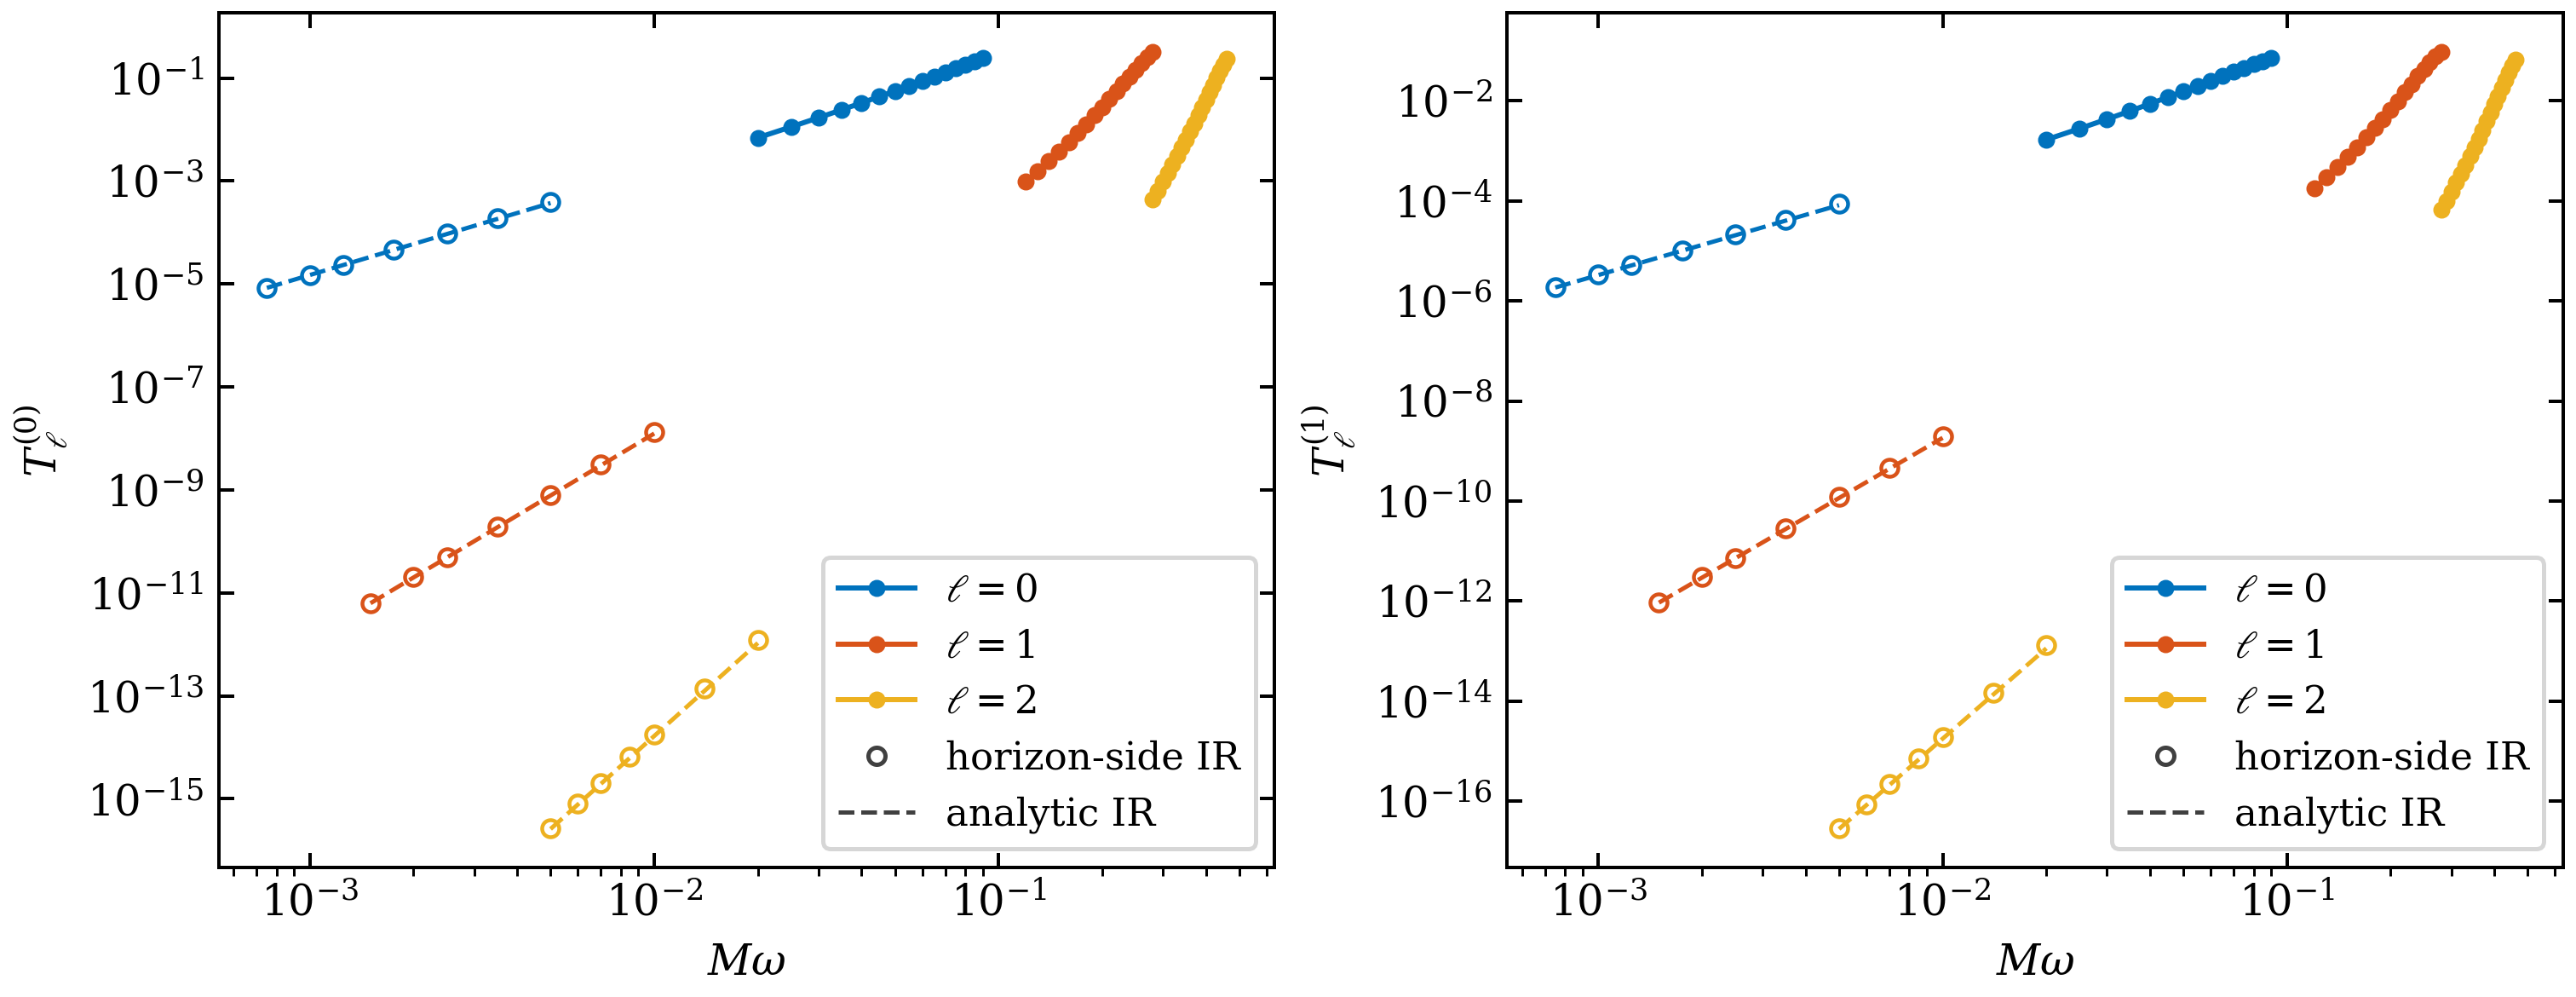
\includegraphics[width=\textwidth]{../../figures/kerr_scalar_low_frequency_axisymmetric.png}
\caption{轴对称三次相互作用的低频吸收。实心点通过两端首阶能流检验；空心点采用更深低频的配对视界侧计算。虚线为式\eqref{eq:T0IR}、\eqref{eq:T1IR}的领先渐近式。两组数据的间隔对应反射干涉项的相消限制。}\label{fig:low}\end{figure}

图\ref{fig:low}中的密集双边数据须满足 $|T^{(1)}+R^{(1)}|\le10^{-8}$。
展示区间为 $\ell=0:[0.02,0.09]$、$\ell=1:[0.12,0.28]$、$\ell=2:[0.28,0.46]$，
分别有 15、17、19 个点；最低点和参数变化见表\ref{note-tab:low-acceptance}、\ref{note-tab:low-convergence}。
改变谱阶、积分阶或匹配半径后，$T^{(1)}$ 最大相对变化为 $1.8\times10^{-8}$。
更深低频处，反射首阶干涉实部由较大复量相消得到，因而先失去精度。空心点只采用直接视界积分及其收敛检验，不以守恒关系重建反射项。幂律拟合使用空心点，而非较高频率的密集展示区间。

\subsection{高次单极相互作用}
对 $n=2,3$，在五个自旋上取七个频率：
\begin{align}
a/M&=(0,0.5,0.9,0.99,0.999),\\
M\omega&=(0.0005,0.00075,0.001,0.0015,0.002,0.003,0.005).
\end{align}
分别用 $(N,q)=(144,144),(176,176)$ 求解。在最低五点对
$\chi_H^{(n)}/\omega^{2n-2}$ 作二次外推，得到领先系数。
改用四点或六点时截距变化不超过 $4.6\times10^{-6}$，跨自旋截距相对标准差为
$1.2\times10^{-6}$ 与 $7.2\times10^{-7}$。
自由拟合指数范围为 $n=2:2.01009$--$2.01016$，$n=3:4.01552$--$4.01561$，
$R^2>0.9999989$，与有限频率修正下的整数极限相符。

另取固定 $y=\omega/\kappa=(0.025,0.05,0.1)$ 的路径，扫描
$a/M=(0.98,0.99,0.995,0.997,0.999)$。
式\eqref{eq:hierarchy}沿这类单极路径对应
\begin{equation}
M^{2n-2}\chi_{H,00}^{(n)}\sim c_n y^{2n-2}(M\kappa)^{2n-2}.
\end{equation}
在 $y=0.025$ 的最高三个自旋处，$\kappa$ 拟合指数为 $2.00734,4.01128$，
$R^2=0.99999988,0.99999993$。这是特定路径上的数值支持，不是极端点的一致渐近证明。
表\ref{note-tab:power-l0}给出系数误差与分辨率变化。

\begin{figure}[htbp]\centering
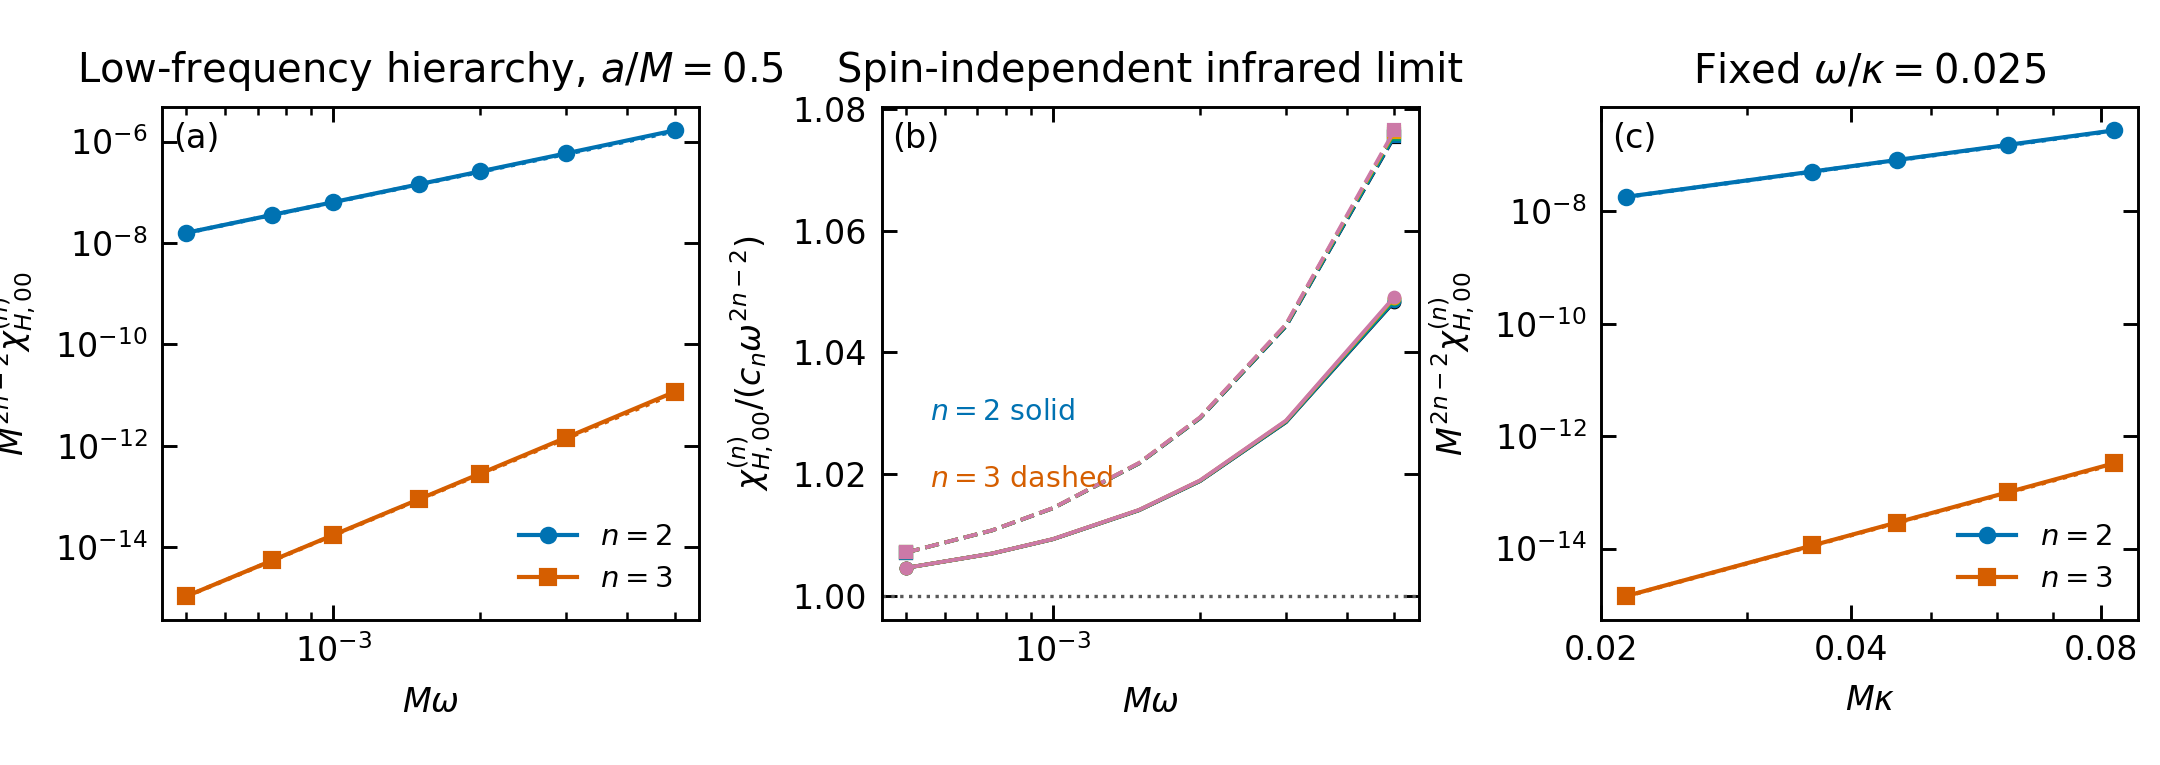
\includegraphics[width=\textwidth]{../../figures/kerr_scalar_power_nonlinearity_l0.png}
\caption{单极高次相互作用的相对响应。左：$n=2,3$ 的直接计算和领先幂律；中：按解析常数缩放的跨自旋比较；右：固定 $\omega/\kappa=0.025$ 时的近极端路径。所有结果均为 $m=0$，不存在超辐射阈值位移。}\label{fig:power}\end{figure}

\subsection{有限频率峰与尾部}
在 $a/M=0.5,m=0$ 的保留样本中，$\ell=0,1,2$ 的 $T^{(1)}$ 均为正。
故式\eqref{eq:model}中 $\epsilon>0$ 时吸收增加、反射减少；通常正四次势能对应 $\epsilon<0$，物理修正方向相反。
图\ref{fig:finite}显示峰与较高频率的衰减。用
\begin{equation}
T^{(1)}=T_{\rm off}+\frac{A\gamma^2}{(M\omega-\omega_p)^2+\gamma^2}
\end{equation}
拟合高于样本峰值 $20\%$ 的点，得到
\begin{align}
\omega_p&=(0.1306,0.3101,0.5026),&\gamma&=(0.0599,0.0591,0.0595),\\
R^2&=(0.9918,0.9978,0.9985).
\end{align}
相应基本标量 QNM 实部为 $(0.1124,0.2979,0.4920)$\cite{Berti2009,Stein2019}，
峰位偏移为 $(16.2,4.1,2.2)\%$。拟合的相对均方根残差为 $(2.41,1.27,1.05)\%$。
将选点门槛改为峰值的 $15\%$--$30\%$ 后，峰中心变化不超过
$(6.7,3.9,3.4)\times10^{-4}$，而宽度更敏感。
这类实频率能流拟合给出 QNM 附近的频率尺度，不计算 QNM 极点或残数；严格的 QNM 投影涉及双线性积和轮廓正则化\cite{GreenEtAl2023}。

\begin{figure}[htbp]\centering
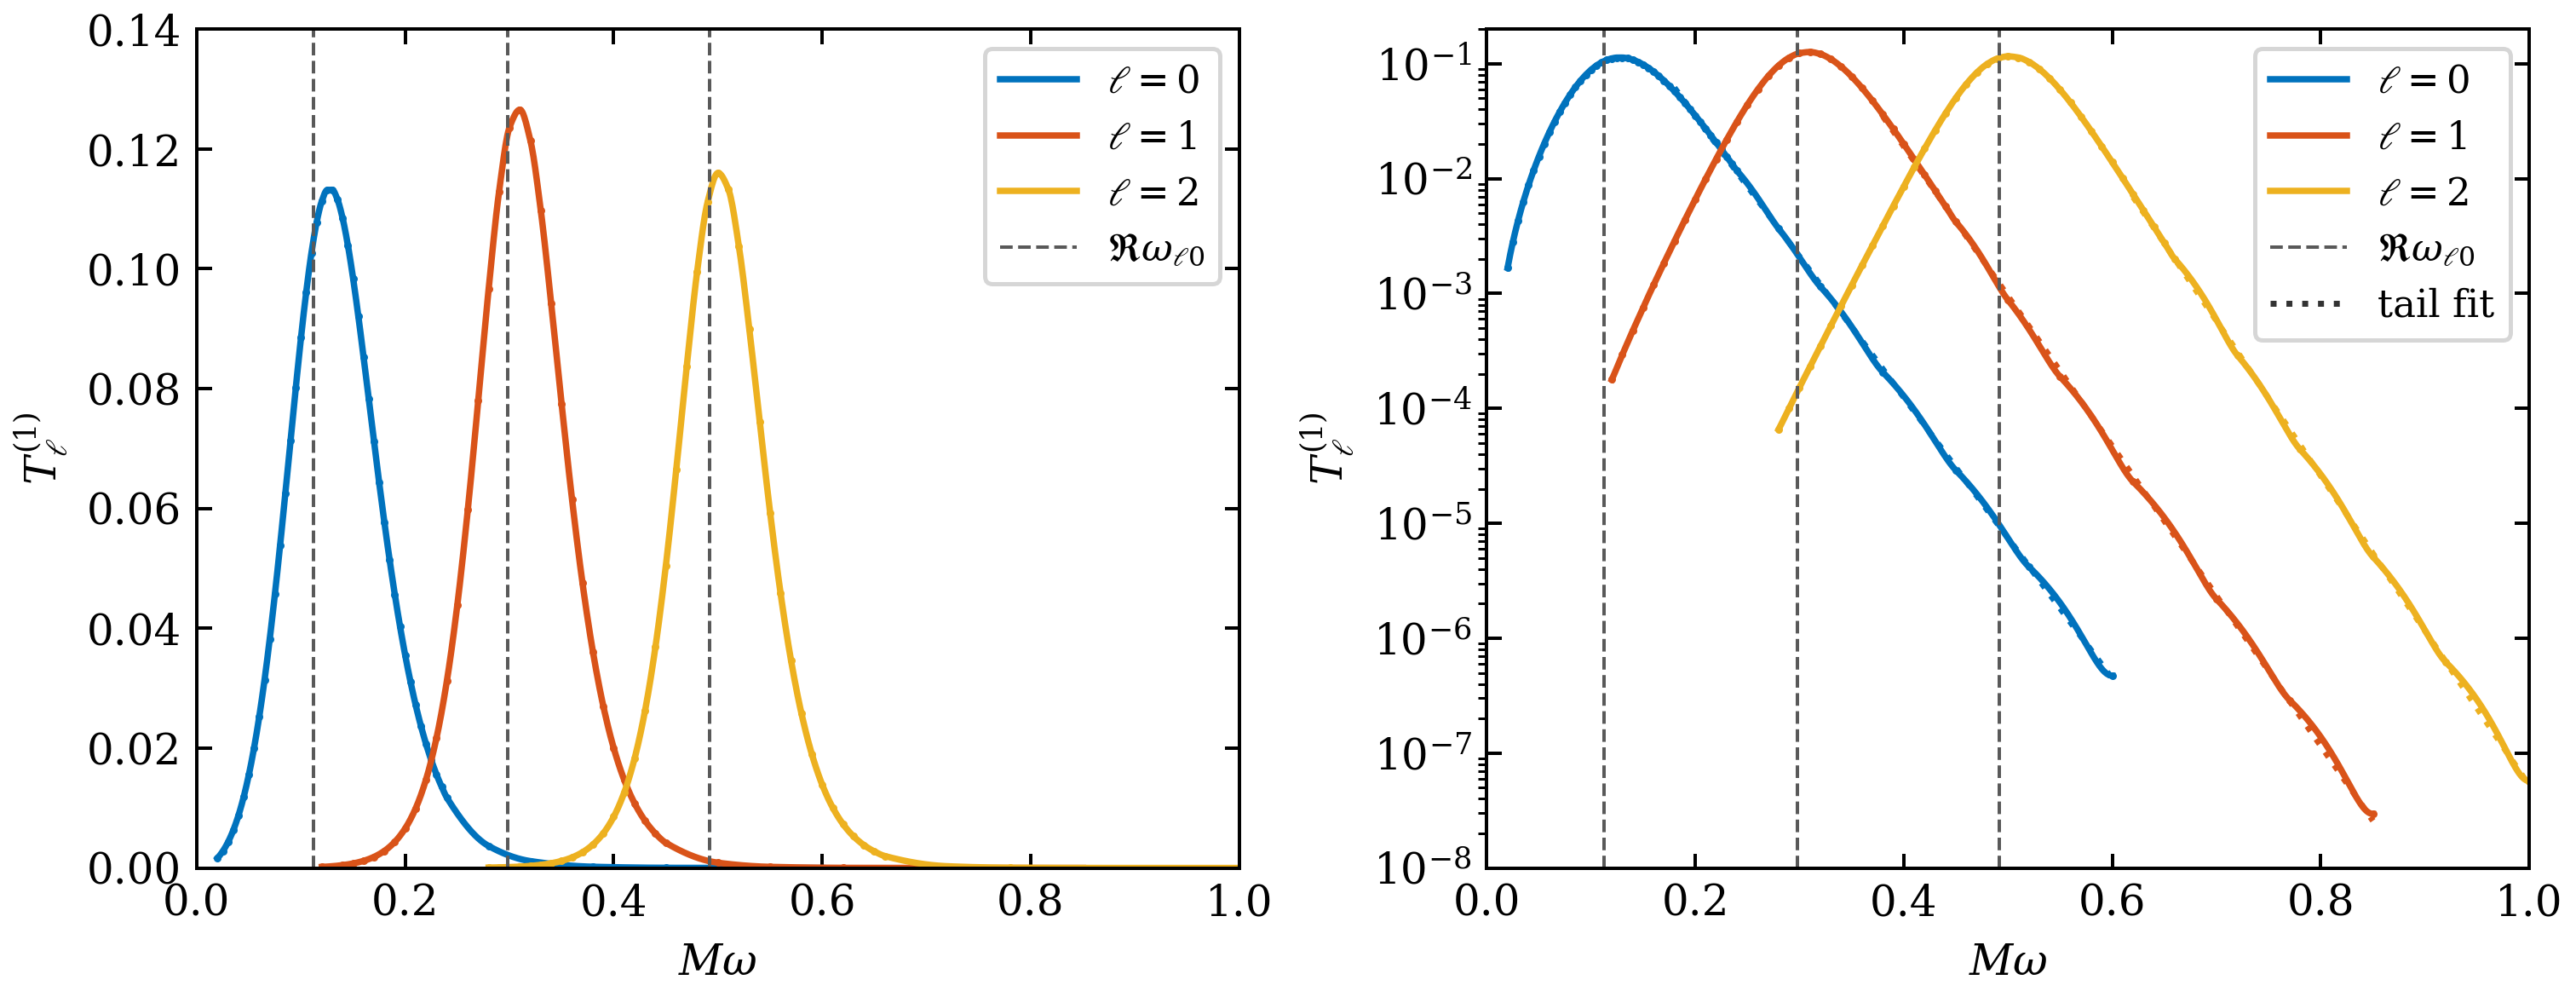
\includegraphics[width=\textwidth]{../../figures/kerr_scalar_nonlinear_axisymmetric_fig2.png}
\caption{有限频率三次透射系数。左图为峰区，右图为指数尾。圆点为实际保留样本，实线为保形插值；竖虚线标记基本标量 QNM 实部。尾拟合共使用 43 个积分阶为 2048 的点。}\label{fig:finite}\end{figure}

尾部拟合使用 $\log T^{(1)}=c-\omega/T_{\rm fit}$，三个窗口分别为
$[0.18,0.60]$、$[0.38,0.85]$、$[0.62,1.00]$，各有 19、14、10 个点。
得到
\begin{equation}\pi MT_{\rm fit}=(0.1114,0.1046,0.1012).\end{equation}
与 Kerr Hawking 温度\cite{Hawking1975}
\begin{equation}
T_H=\frac{r_+-r_-}{4\pi(r_+^2+a^2)},\qquad \pi MT_H=0.1160\quad(a/M=0.5)
\end{equation}
相比，偏差为 $4.00\%,9.85\%,12.81\%$。这是灰体因子研究中有限窗口热尺度诊断\cite{Oshita2023,Oshita2024}，不是由本经典方程推导热辐射。
移动窗口后的结果见表\ref{note-tab:tail-window}。

在相同点上比较两个两参数模型 $c-\beta M\omega$ 与 $c-\nu\log(M\omega)$，使用小样本修正的 Akaike 信息准则
\begin{equation}
\mathrm{AICc}=n_s\log(\mathrm{RSS}/n_s)+2k+\frac{2k(k+1)}{n_s-k-1},\qquad k=2.
\end{equation}
指数模型相对于幂律模型的 $\Delta\mathrm{AICc}$ 为 $97.9,48.2,23.8$，留一预测残差也更小。
若固定指数斜率为 $-1/T_H$，对数空间的均方根残差增至 $0.139,0.443,0.514$。
因而数据支持这些窗口中的指数描述，而不支持将其斜率严格等同于 Hawking 温度。全部拟合和模型比较见表\ref{note-tab:fit}、\ref{note-tab:tail-models}。

\subsection{自旋连续性与数值误差}
固定 $(\ell,m,M\omega)=(2,0,0.52)$，逐点重算
$a/M=0,0.05,0.1,0.2,0.3,0.5$。
$T^{(1)}$ 由 $0.0894395$ 平滑增至 $0.103814$，与 $-R^{(1)}$ 一致，如图\ref{fig:spin}和表\ref{note-tab:spin-limit}。
有限频率的自旋依赖不与式\eqref{eq:rhoIR}矛盾：后者只约束固定自旋低频极限的相对响应。

\begin{figure}[htbp]\centering
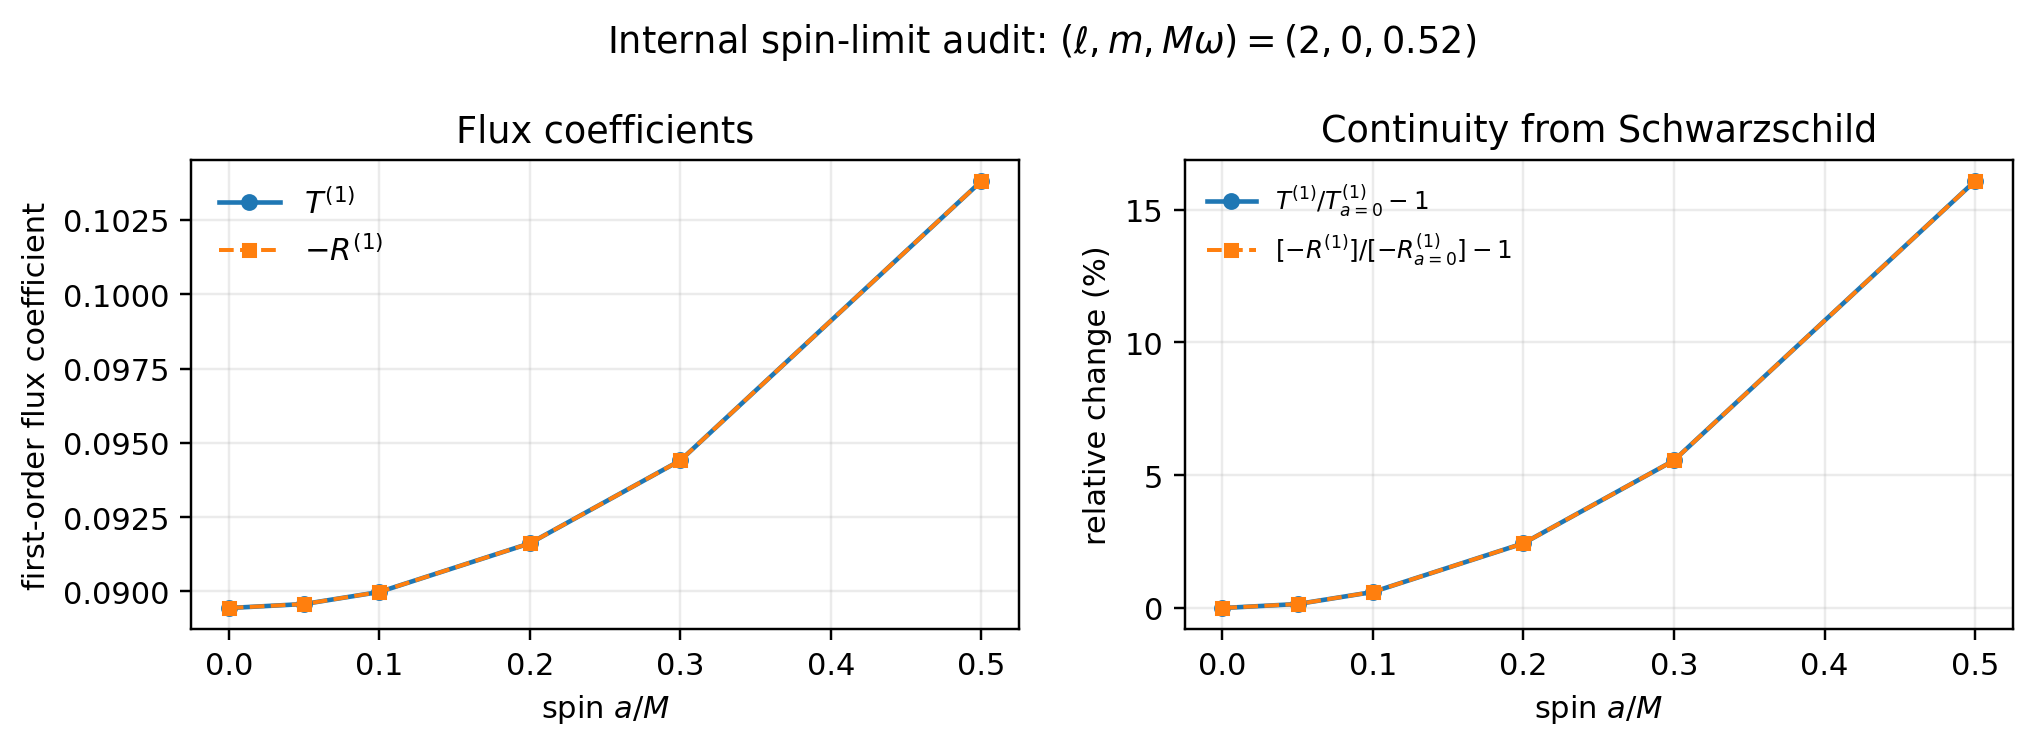
\includegraphics[width=\textwidth]{../../figures/kerr_scalar_spin_limit.png}
\caption{固定 $(\ell,m,M\omega)=(2,0,0.52)$ 的自旋连续性。左：两端首阶系数；右：除以 $a=0$ 的值。整个扫描使用同一固定入射归一化与包含端点的谱方程。}\label{fig:spin}\end{figure}

角离散审计中，本征值相对变化不超过 $4.4\times10^{-16}$，源投影不超过 $5.3\times10^{-14}$。
径向误差随频率区间而不同。代表峰点
$(a,\ell,m,M\omega)=(0.5,2,0,0.52)$ 的 1800 个独立齐次验证点给出残差最大值、95\% 分位数和中位数
$2.8\times10^{-10},1.2\times10^{-11},3.2\times10^{-13}$，最大谱尾 $2.8\times10^{-14}$。
图\ref{fig:accuracy}显示这些诊断。峰区生产配置从 $(N,q)=(224,160)$ 改为 $(240,192)$ 时，
$T^{(1)}$ 变化最多 $3.1\times10^{-5}$，尽管两端流平衡达到 $10^{-12}$。

\begin{figure}[htbp]\centering
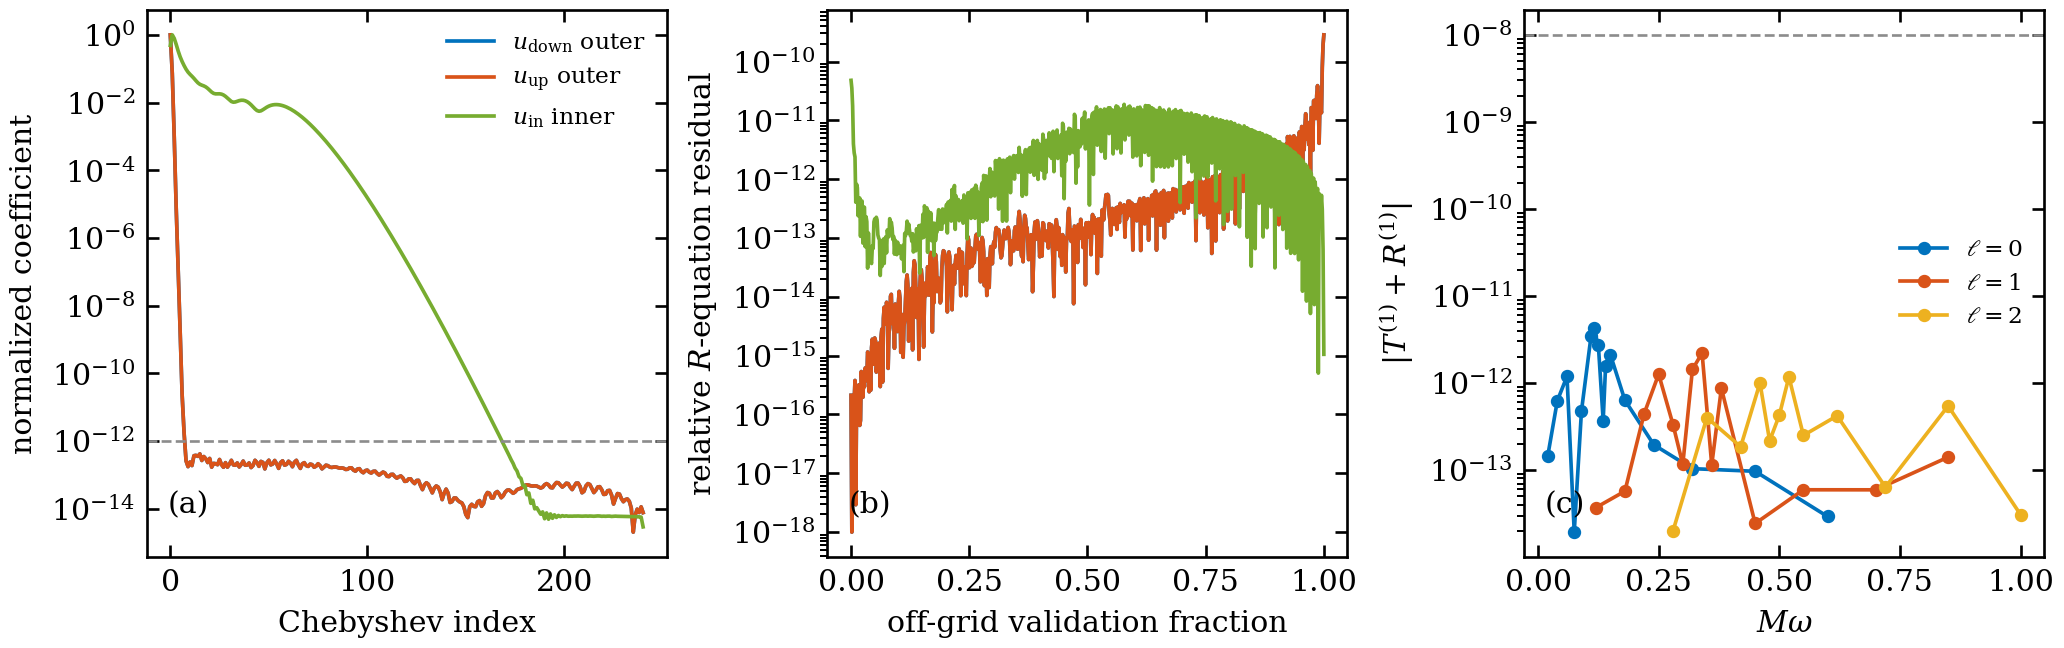
\includegraphics[width=\textwidth]{../../figures/kerr_scalar_axisymmetric_accuracy.png}
\caption{齐次解的谱系数、独立径向残差和首阶能流误差。前两项取代表峰点，第三项覆盖保留的轴对称数据。虚线为展示数据的首阶能流门槛 $10^{-8}$。}\label{fig:accuracy}\end{figure}

较高频率尾部的主要敏感性来自 Green 积分。固定 $N=240$，$q=1792\to2048$ 时，
$T^{(1)}$ 的相对变化最多 $2.5\times10^{-4}$；固定 $q=2048$ 改变谱阶的影响明显较小。
两类变化见表\ref{note-tab:production-convergence}、\ref{note-tab:tail-convergence}。
主曲线保留点数为 $51,40,44$，两端首阶能流最大误差为
$6.9\times10^{-12},2.2\times10^{-12},1.5\times10^{-12}$，见表\ref{note-tab:numerics}。

深低频高次单极代表点 $(a/M,M\omega,N)=(0.5,5\times10^{-4},176)$ 的谱尾不超过
$5.2\times10^{-14}$，但原方程残差最大值为 $1.6\times10^{-5}$，95\% 分位数为 $2.1\times10^{-7}$，中位数为 $2.7\times10^{-10}$。
对应响应仍通过配对分辨率检验，不能据此声称整个径向域统一达到机器精度。

对有源场的独立验证在 $[3M,8M]$ 上进行，齐次谱阶为 224，重构阶为 $D=16,24,32,48,64$。
A、B 取 $a=.5,\ell=m=0,M\omega=.1$，分别为 $n=1,2$；C 取
$a=.99,\ell=m=2,p/\kappa=.5,n=1$。
重构积分中视界至 $3M$ 使用 1024 点，局域增量使用 128 点，残差在 600 个独立节点计算。
在 $D=32$，三例的最大有源残差均低于 $2.3\times10^{-9}$；更高阶出现非单调误差底，见图\ref{fig:sourced}和表\ref{note-tab:sourced20261008}。
这检验所述内区的局域方程，不检验全部渐近区或累积积分常数。

\begin{figure}[htbp]\centering
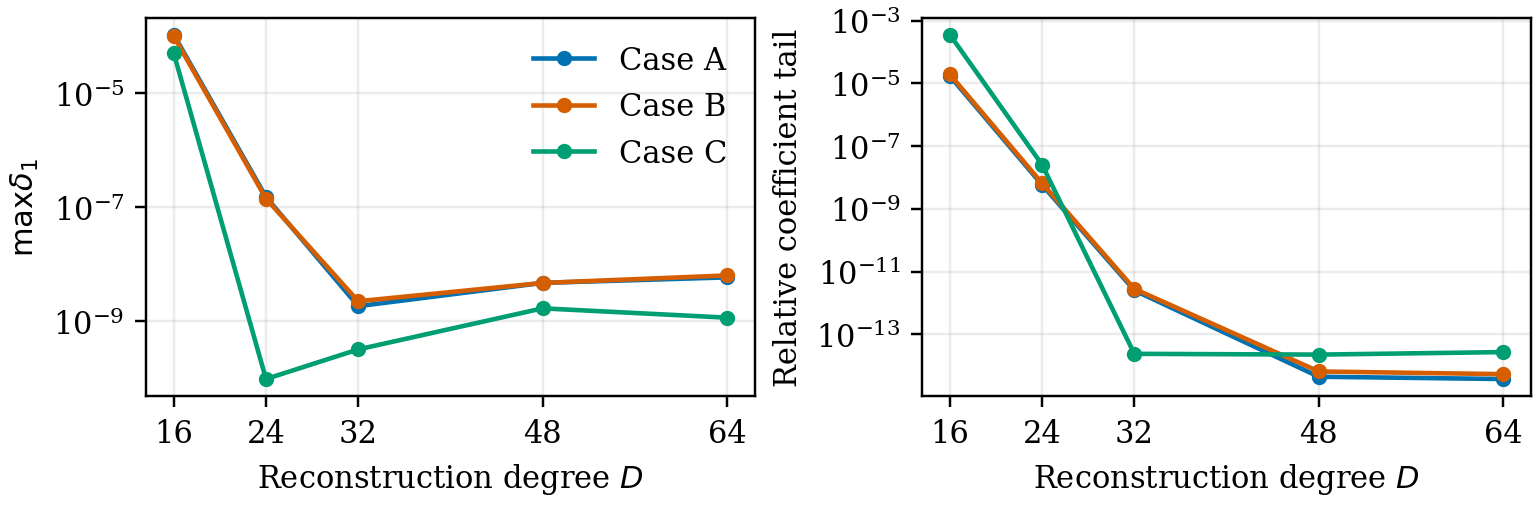
\includegraphics[width=\textwidth]{../../figures/kerr_scalar_sourced_local_validation_20261008.png}
\caption{有源场的独立局域重构。左：式\eqref{eq:sourceres}的最大残差；右：最后八个重构谱系数的相对尾部。低阶截断误差下降后出现数值微分误差底，谱尾继续减小不保证残差单调改善。}\label{fig:sourced}\end{figure}

\section{讨论}
三次轴对称散射的主要解析结果是式\eqref{eq:T0IR}和式\eqref{eq:T1IR}：绝对吸收与首阶系数按相同的角势垒幂次消失，因此相对响应保留有限极限。
其领先自旋独立性来自 Green 源积分与入射归一化中的近区匹配系数抵消，并不意味着有限频率的吸收不受旋转影响。
单极复响应的虚部还给出能流中没有包含的相位信息。
更一般的单极局域作用由式\eqref{eq:hierarchy}区分：三次项保留有限相对响应，而高次项以 $2n-2$ 次幂受抑制。
相应正性由式\eqref{eq:positive}证明，$n=2,3$ 的跨自旋实验分别检验了系数和指数。

近极端问题需要另行处理。固定 $a$ 的 $\omega\to0$、固定 $a$ 的 $p\to0$，以及固定 $p/\kappa$ 的 $\kappa\to0$ 不是同一极限。
对 $m\ne0$，最后一条路径满足 $\omega=m\Omega_H+y\kappa$，趋于超辐射阈值而非零频率。
Kerr/CFT 的线性近视界吸收因子\cite{BredbergKerrCFT2010}不能单独确定非线性响应的指数，因为后者还包含完整源积分、Green 核与远区归一化。
当前结果没有建立非轴对称 principal 模态的普遍 $\kappa^{-1}$ 或 $\kappa^{2\Rea h-2}$ 定律。

非轴对称求解器已作有限参数检查：$a/M=.99,.999$、$\ell=m=1,2$、$n=1,2$、$p/\kappa=.5$。
外端行采用正确的 $B_0(0)=-\lambda-2am\omega$，并先消去剥离方程中的表观奇异项。
该组齐次原方程残差最大为 $3.2\times10^{-9}$，剥离方程残差最大为 $5.2\times10^{-8}$。
这些测试不构成近极端幂律拟合，也不足以验证全部历史非轴对称扫描。

进一步研究包括完整模式耦合的首阶场、二阶能流、近极端一致匹配以及时间域的扰动有效性。
本文未计算非线性饱和或引力反作用。有限频率的峰和指数尾应分别作为实轴共振尺度与有限窗口衰减规律解释。
数值方面，局域场残差、积分收敛与两端能流仍需分别控制，不能由单一守恒误差给出统一精度。

\FloatBarrier
\appendix
\section{数值表}
本附录保留现行稿件的全部数值表。表中的 $N$ 是径向谱阶，$q$ 是 Green 积分阶；
表中首阶系数按式\eqref{eq:T1}、\eqref{eq:Ref1}或其高次推广定义。
\begin{table}[htbp]
\centering
\caption{角向离散审计：本征值和两个源投影相对于额外 24 个基与 512 点参考配置的最大相对变化。}
\label{note-tab:angular-convergence}
\begin{adjustbox}{max width=\textwidth}
\begin{tabular}{lccc}
setting $(L_{\rm extra},q_\theta)$ & $\max\Delta\lambda$
& $\max\Delta C^{(0)}$ & $\max\Delta C^{(2)}$\\
\midrule
active $(16,256)$ & $4.4\times10^{-16}$ & $3.7\times10^{-14}$ & $5.2\times10^{-14}$\\
basis $(12,512)$ & $4.4\times10^{-16}$ & $1.6\times10^{-16}$ & $0$\\
quadrature $(24,128)$ & $0$ & $1.5\times10^{-14}$ & $2.0\times10^{-14}$\\
\end{tabular}
\end{adjustbox}
\end{table}

\begin{table}[htbp]
\centering
\caption{三次轴对称红外解析系数及直接视界侧检验，$a/M=0.5$。最后一列比较两组谱阶和积分阶。}
\label{note-tab:axisymmetric-infrared}
\begin{adjustbox}{max width=\textwidth}
\begin{tabular}{c c c c c c c}
$\ell$ & ${\cal I}_\ell$ & $\chi^{\rm IR}_\ell$
& ${\cal A}^{(0)}_\ell$ & ${\cal A}^{(1)}_\ell$
& lowest $M\omega$ & $\delta_N\chi_H$\\
\hline
0 & 0.346573590280 & 0.220635600153 & 14.9282032 & 3.29369308 & 0.00075 & $1.1\times10^{-7}$\\
1 & 0.128401008797 & 0.147136717786 & 1.24401694 & 0.183040569 & 0.00150 & $1.5\times10^{-4}$\\
2 & 0.077970747421 & 0.106366541731 & 0.0165868925 & 0.00176429039 & 0.00500 & $7.7\times10^{-5}$\\
\end{tabular}
\end{adjustbox}
\end{table}

\begin{table}[htbp]
\centering
\caption{通过双边首阶能流门槛的低频展示区间、点数和最低点的实际结果。}
\label{note-tab:low-acceptance}
\begin{adjustbox}{max width=\textwidth}
\begin{tabular}{c c c c c c}
$\ell$ & displayed $M\omega$ range & points
& $T^{(0)}_{\rm low}$ & $T^{(1)}_{\rm low}$ & $|\delta_1|_{\rm low}$\\
\hline
0 & $[0.02,0.09]$ & 15 & $6.92348\times10^{-3}$ & $1.67885\times10^{-3}$ & $1.4\times10^{-13}$\\
1 & $[0.12,0.28]$ & 17 & $9.73095\times10^{-4}$ & $1.78519\times10^{-4}$ & $3.7\times10^{-14}$\\
2 & $[0.28,0.46]$ & 19 & $4.35440\times10^{-4}$ & $6.58814\times10^{-5}$ & $2.0\times10^{-14}$\\
\end{tabular}
\end{adjustbox}
\end{table}

\begin{table}[htbp]
\centering
\caption{各多极最低展示点的独立参数审计：改变谱阶、积分阶或匹配半径，相对参考 $(256,256,40)$ 比较。}
\label{note-tab:low-convergence}
\begin{adjustbox}{max width=\textwidth}
\begin{tabular}{c c c c c c}
$\ell$ & $M\omega$ & $T^{(1)}_{\rm ref}$
& $\max|\Delta T^{(1)}/T^{(1)}|$
& $\max|\Delta R^{(1)}/R^{(1)}|$ & $\max|\delta_1|$\\
\hline
0 & 0.02 & $1.67885\times10^{-3}$ & $1.8\times10^{-8}$ & $2.0\times10^{-8}$ & $3.0\times10^{-12}$\\
1 & 0.12 & $1.78519\times10^{-4}$ & $6.7\times10^{-9}$ & $7.3\times10^{-9}$ & $3.8\times10^{-13}$\\
2 & 0.28 & $6.58814\times10^{-5}$ & $9.2\times10^{-9}$ & $4.6\times10^{-9}$ & $2.8\times10^{-13}$\\
\end{tabular}
\end{adjustbox}
\end{table}

\begin{table}[htbp]
\centering
\caption{单极高次作用的解析常数、拟合指数、外推系数误差与双分辨率变化；固定 $y$ 为 $y=0.025$。}
\label{note-tab:power-l0}
\begin{adjustbox}{max width=\textwidth}
\begin{tabular}{c c c c c c c}
$n$ & $c_n$ & predicted power & fixed-$\omega$ fitted power
& fixed-$y$ $\kappa$ power & max. coefficient error & max. $\delta_N\chi_H$\\
\hline
2 & 0.0631722552 & 2 & 2.01009--2.01016 & 2.00734 & $2.8\times10^{-6}$ & $2.5\times10^{-6}$\\
3 & 0.0172436384 & 4 & 4.01552--4.01561 & 4.01128 & $1.3\times10^{-6}$ & $7.7\times10^{-9}$\\
\end{tabular}
\end{adjustbox}
\end{table}

\begin{table}[htbp]
\centering
\caption{有限频率峰和指数尾的现象学拟合参数。QNM 为基本标量模，频率单位 $M=1$；$\Delta T$ 是与 Hawking 温度的相对偏差。}
\label{note-tab:fit}
\begin{adjustbox}{max width=\textwidth}
\begin{tabular}{c c c c c c c}
$\ell$ & $\omega_p$ & $\gamma$
& $\Re\omega_Q$
& $|\Im\omega_Q|$
& $\pi T_{\rm fit}$
& $\Delta T$\\
\hline
0 & 0.1306 & 0.0599 & 0.1124 & 0.1022 & 0.1114 & 4.00\%\\
1 & 0.3101 & 0.0591 & 0.2979 & 0.0954 & 0.1046 & 9.85\%\\
2 & 0.5026 & 0.0595 & 0.4920 & 0.0946 & 0.1012 & 12.81\%\\
\end{tabular}
\end{adjustbox}
\end{table}

\begin{table}[htbp]
\centering
\caption{移动指数尾拟合窗口后的有效温度范围、log 残差与温度偏差；不是无限高频误差界。}
\label{note-tab:tail-window}
\begin{adjustbox}{max width=\textwidth}
\begin{tabular}{c c c c c c}
$\ell$ & baseline $[M\omega_{\min},M\omega_{\max}]$
& $\pi T_{\rm fit}^{\rm base}$ & range of $\pi T_{\rm fit}$
& $\max\sigma_{\log}$ & $\max|T_{\rm fit}/T_H-1|$\\
\hline
0 & $[0.18,0.60]$ & 0.1114 & $[0.1109,0.1122]$ & $3.86\times10^{-2}$ & 4.45\%\\
1 & $[0.38,0.85]$ & 0.1046 & $[0.1037,0.1068]$ & $6.95\times10^{-2}$ & 10.61\%\\
2 & $[0.62,1.00]$ & 0.1012 & $[0.1002,0.1031]$ & $5.59\times10^{-2}$ & 13.62\%\\
\end{tabular}
\end{adjustbox}
\end{table}

\begin{table}[htbp]
\centering
\caption{指数与幂律尾的同参数数目比较。正的 $\Delta\mathrm{AICc}$ 支持指数模型，LOO 为留一预测误差。}
\label{note-tab:tail-models}
\begin{adjustbox}{max width=\textwidth}
\begin{tabular}{c c c c c c c}
$\ell$ & points & $\sigma_{\rm exp}$ & $\sigma_{\rm power}$
& $\Delta\mathrm{AICc}$ & $\sigma_{\rm LOO,exp}$ & $\sigma_{\rm LOO,power}$\\
\hline
0 & 19 & $3.72\times10^{-2}$ & $4.89\times10^{-1}$ & 97.9 & $4.56\times10^{-2}$ & $6.09\times10^{-1}$\\
1 & 14 & $6.71\times10^{-2}$ & $3.75\times10^{-1}$ & 48.2 & $8.92\times10^{-2}$ & $4.80\times10^{-1}$\\
2 & 10 & $5.59\times10^{-2}$ & $1.84\times10^{-1}$ & 23.8 & $8.11\times10^{-2}$ & $2.62\times10^{-1}$\\
\end{tabular}
\end{adjustbox}
\end{table}

\begin{table}[htbp]
\centering
\caption{轴对称扫描的保留点数和两种能流误差。低频及峰区 $q=192$，尾拟合 43 点 $q=2048$，谱阶均为 240。}
\label{note-tab:numerics}
\begin{adjustbox}{max width=\textwidth}
\begin{tabular}{c c c c c c}
$\ell$ & retained & $M\omega_{\min}$ & $\max\delta_0$ & $\max\delta_1$
& $\sigma_{\rm tail}$\\
\hline
0 & 51 & 0.02 & $2.8\times10^{-11}$ & $6.9\times10^{-12}$ & $3.7\times10^{-2}$\\
1 & 40 & 0.12 & $1.9\times10^{-11}$ & $2.2\times10^{-12}$ & $6.7\times10^{-2}$\\
2 & 44 & 0.28 & $3.8\times10^{-11}$ & $1.5\times10^{-12}$ & $5.6\times10^{-2}$\\
\end{tabular}
\end{adjustbox}
\end{table}

\begin{table}[htbp]
\centering
\caption{旧生产配置 $(224,160)$ 与当前峰区配置 $(240,192)$ 的相对变化。小守恒误差不代表两配置完全一致。}
\label{note-tab:production-convergence}
\begin{adjustbox}{max width=\textwidth}
\begin{tabular}{c c c c c c}
case & $\Delta A_{\rm ref}$ & $\Delta A_H$
& $\Delta T^{(1)}$ & $\Delta R^{(1)}$ & $|\delta_1|_{\rm ref}$\\
\hline
$\ell=0,\ M\omega=.125$ & $4.5\times10^{-7}$ & $7.8\times10^{-7}$
& $2.3\times10^{-6}$ & $2.3\times10^{-6}$ & $2.7\times10^{-12}$\\
$\ell=1,\ M\omega=.34$ & $5.9\times10^{-6}$ & $3.3\times10^{-6}$
& $1.5\times10^{-5}$ & $1.5\times10^{-5}$ & $2.2\times10^{-12}$\\
$\ell=2,\ M\omega=.52$ & $9.6\times10^{-6}$ & $7.6\times10^{-6}$
& $3.1\times10^{-5}$ & $3.1\times10^{-5}$ & $1.2\times10^{-12}$\\
\end{tabular}
\end{adjustbox}
\end{table}

\begin{table}[htbp]
\centering
\caption{尾区独立积分阶及谱阶审计。积分阶比较 1792 与 2048；谱阶比较 224 与 240。}
\label{note-tab:tail-convergence}
\begin{adjustbox}{max width=\textwidth}
\begin{tabular}{c c c c c c}
case & $\Delta T^{(1)}[q]$ & $\Delta T^{(1)}[N]$
& $\Delta A_{\rm ref}[q]$ & $\Delta A_H[q]$ & $|\delta_1|_{\rm ref}$\\
\hline
$\ell=0,\ M\omega=.52$ & $3.0\times10^{-5}$ & $7.1\times10^{-10}$ & $2.3\times10^{-5}$ & $1.6\times10^{-9}$ & $7.8\times10^{-15}$\\
$\ell=1,\ M\omega=.77$ & $1.7\times10^{-4}$ & $1.0\times10^{-9}$ & $3.1\times10^{-4}$ & $1.2\times10^{-9}$ & $2.7\times10^{-13}$\\
$\ell=2,\ M\omega=.92$ & $2.5\times10^{-4}$ & $9.5\times10^{-8}$ & $3.4\times10^{-4}$ & $2.5\times10^{-9}$ & $1.0\times10^{-14}$\\
\end{tabular}
\end{adjustbox}
\end{table}

\begin{table}[htbp]
\centering
\caption{固定 $(\ell,m,M\omega)=(2,0,0.52)$ 的 Kerr 到施瓦西连续性检查。}
\label{note-tab:spin-limit}
\begin{adjustbox}{max width=\textwidth}
\begin{tabular}{c c c c c c}
$a/M$ & $T^{(1)}$ & $R^{(1)}$ & $|\delta_0|$ & $|\delta_1|$ & $|\delta_W|$\\
\hline
0.00 & $8.94395\times10^{-2}$ & $-8.94395\times10^{-2}$ & $1.1\times10^{-12}$ & $3.8\times10^{-13}$ & $2.6\times10^{-16}$\\
0.05 & $8.95742\times10^{-2}$ & $-8.95742\times10^{-2}$ & $9.8\times10^{-12}$ & $1.1\times10^{-12}$ & $3.3\times10^{-16}$\\
0.10 & $8.99794\times10^{-2}$ & $-8.99794\times10^{-2}$ & $3.7\times10^{-12}$ & $4.9\times10^{-13}$ & $0$\\
0.20 & $9.16178\times10^{-2}$ & $-9.16178\times10^{-2}$ & $4.3\times10^{-13}$ & $7.6\times10^{-14}$ & $1.8\times10^{-16}$\\
0.30 & $9.44095\times10^{-2}$ & $-9.44095\times10^{-2}$ & $1.1\times10^{-11}$ & $1.3\times10^{-12}$ & $1.8\times10^{-16}$\\
0.50 & $1.03814\times10^{-1}$ & $-1.03814\times10^{-1}$ & $6.0\times10^{-12}$ & $1.2\times10^{-12}$ & $0$\\
\end{tabular}
\end{adjustbox}
\end{table}

\begin{table}[htbp]
\centering
\caption{完整局域有源残差阶数扫描。A、B 为单极三次和五次作用，C 为非轴对称求解器探针；尾为最后八个重构系数的相对最大模。}
\label{note-tab:sourced20261008}
\begin{adjustbox}{max width=\textwidth}
\begin{tabular}{ccccc}
Case & $D$ & $\max\delta_1$ & median $\delta_1$ & tail\\
A & 16 & $1.05\times10^{-4}$ & $4.11\times10^{-6}$ & $1.71\times10^{-5}$\\
A & 24 & $1.52\times10^{-7}$ & $3.97\times10^{-9}$ & $5.78\times10^{-9}$\\
A & 32 & $1.85\times10^{-9}$ & $1.31\times10^{-11}$ & $2.50\times10^{-12}$\\
A & 48 & $4.73\times10^{-9}$ & $3.36\times10^{-11}$ & $4.42\times10^{-15}$\\
A & 64 & $5.90\times10^{-9}$ & $5.51\times10^{-11}$ & $3.74\times10^{-15}$\\
B & 16 & $9.87\times10^{-5}$ & $3.63\times10^{-6}$ & $1.93\times10^{-5}$\\
B & 24 & $1.42\times10^{-7}$ & $3.50\times10^{-9}$ & $6.50\times10^{-9}$\\
B & 32 & $2.25\times10^{-9}$ & $1.64\times10^{-11}$ & $2.81\times10^{-12}$\\
B & 48 & $4.71\times10^{-9}$ & $3.69\times10^{-11}$ & $6.51\times10^{-15}$\\
B & 64 & $6.38\times10^{-9}$ & $6.47\times10^{-11}$ & $5.35\times10^{-15}$\\
C & 16 & $4.97\times10^{-5}$ & $5.87\times10^{-7}$ & $3.56\times10^{-4}$\\
C & 24 & $9.77\times10^{-11}$ & $2.37\times10^{-12}$ & $2.54\times10^{-8}$\\
C & 32 & $3.23\times10^{-10}$ & $2.22\times10^{-12}$ & $2.38\times10^{-14}$\\
C & 48 & $1.69\times10^{-9}$ & $6.69\times10^{-12}$ & $2.24\times10^{-14}$\\
C & 64 & $1.16\times10^{-9}$ & $1.29\times10^{-11}$ & $2.70\times10^{-14}$\\
\end{tabular}
\end{adjustbox}
\end{table}

\FloatBarrier
\section{资料来源}
原稿为 Jing-Qi Lai 与 Yu Tian 的 \emph{Infrared hierarchy of nonlinear scalar absorption by Kerr black holes}，
本地源文件为 \nolinkurl{docs/prd/kerr_scalar_nonlinear_prd_review_20261007.tex}，含 2026 年 10 月 8 日的验证附录。
计算验证记录见 \nolinkurl{docs/prd/PRD_VALIDATION_20261008.md}；有源重构数据见
\nolinkurl{results/kerr_scalar_sourced_local_residual_20261008.csv}。
参考施瓦西稿件\cite{HeTianZhangManuscript2026}是作者提供的稿本，并非已核实的正式发表版本。
\begin{thebibliography}{99}
\bibitem{Sanchez1976}
N.~G. Sanchez,
Scattering of scalar waves from a Schwarzschild black hole,
J. Math. Phys. \textbf{17}, 688 (1976).

\bibitem{Futterman}
J.~A. H. Futterman, F.~A. Handler, and R.~A. Matzner,
\textit{Scattering from Black Holes}
(Cambridge University Press, Cambridge, 1988).

\bibitem{GlampedakisAndersson2001}
K.~Glampedakis and N.~Andersson,
Scattering of scalar waves by rotating black holes,
Class. Quantum Grav. \textbf{18}, 1939 (2001).

\bibitem{Berti2009}
E.~Berti, V.~Cardoso, and A.~O. Starinets,
Quasinormal modes of black holes and black branes,
Class. Quantum Grav. \textbf{26}, 163001 (2009).

\bibitem{Kyutoku2023}
K.~Kyutoku, H.~Motohashi, and T.~Tanaka,
Quasinormal modes of Schwarzschild black holes on the real axis,
Phys. Rev. D \textbf{107}, 044012 (2023).

\bibitem{Rosato2024}
R.~F. Rosato, K.~Destounis, and P.~Pani,
Ringdown stability: Graybody factors as stable gravitational-wave observables,
Phys. Rev. D \textbf{110}, L121501 (2024).

\bibitem{Zlochower2003}
Y.~Zlochower, R.~G\'omez, S.~Husa, L.~Lehner, and J.~Winicour,
Mode coupling in the nonlinear response of black holes,
Phys. Rev. D \textbf{68}, 084014 (2003),
doi:10.1103/PhysRevD.68.084014,
arXiv:gr-qc/0306098.

\bibitem{Frauendiener2021}
J.~Frauendiener and C.~Stevens,
The non-linear perturbation of a black hole by gravitational waves. I. The
Bondi-Sachs mass loss,
Class. Quantum Grav. \textbf{38}, 194002 (2021).

\bibitem{YoshinoKodama2012}
H.~Yoshino and H.~Kodama,
Bosenova collapse of axion cloud around a rotating black hole,
Prog. Theor. Phys. \textbf{128}, 153 (2012),
doi:10.1143/PTP.128.153,
arXiv:1203.5070 [gr-qc].

\bibitem{Baryakhtar2021}
M.~Baryakhtar, M.~Galanis, R.~Lasenby, and O.~Simon,
Black hole superradiance of self-interacting scalar fields,
Phys. Rev. D \textbf{103}, 095019 (2021),
doi:10.1103/PhysRevD.103.095019,
arXiv:2011.11646 [hep-ph].

\bibitem{HerdeiroQCloud2014}
C.~Herdeiro, E.~Radu, and H.~R\'unarsson,
Non-linear $Q$-clouds around Kerr black holes,
Phys. Lett. B \textbf{739}, 302 (2014),
doi:10.1016/j.physletb.2014.11.005,
arXiv:1409.2877 [gr-qc].

\bibitem{BarackPound2019}
L.~Barack and A.~Pound,
Self-force and radiation reaction in general relativity,
Rep. Prog. Phys. \textbf{82}, 016904 (2019).

\bibitem{PoundWardell2021}
A.~Pound and B.~Wardell,
Black hole perturbation theory and gravitational self-force,
in \textit{Handbook of Gravitational Wave Astronomy}, edited by
C.~Bambi (Springer, Singapore, 2021), Chap.~38,
doi:10.1007/978-981-15-4702-7\_38-1,
arXiv:2101.04592 [gr-qc].

\bibitem{HeTianZhangManuscript2026}
Z.-T. He, Y. Tian, and H. Zhang,
Nonlinear scattering problem in black hole spacetimes,
supplied manuscript, version dated June 15, 2026.
\bibitem{BredbergKerrCFT2010}
I.~Bredberg, T.~Hartman, W.~Song, and A.~Strominger,
Black hole superradiance from Kerr/CFT,
J. High Energy Phys. \textbf{04} (2010) 019,
doi:10.1007/JHEP04(2010)019,
arXiv:0907.3477 [hep-th].

\bibitem{Teukolsky1973}
S.~A. Teukolsky,
Perturbations of a rotating black hole. I. Fundamental equations for
gravitational, electromagnetic, and neutrino-field perturbations,
Astrophys. J. \textbf{185}, 635 (1973).

\bibitem{MST1996}
S.~Mano, H.~Suzuki, and E.~Takasugi,
Analytic solutions of the Teukolsky equation and their low frequency
expansions,
Prog. Theor. Phys. \textbf{95}, 1079 (1996),
arXiv:gr-qc/9603020.

\bibitem{ChungWagleYunes2023}
A.~K.-W. Chung, P.~Wagle, and N.~Yunes,
Spectral method for the gravitational perturbations of black holes:
Schwarzschild background case,
Phys. Rev. D \textbf{107}, 124032 (2023),
arXiv:2302.11624 [gr-qc].

\bibitem{Hughes2000}
S.~A. Hughes,
Computing radiation from Kerr black holes: Generalization of the
Sasaki--Nakamura equation,
Phys. Rev. D \textbf{61}, 084004 (2000),
arXiv:gr-qc/0002043.

\bibitem{Lo2023}
R.~K.~L. Lo,
Recipes for computing radiation from a Kerr black hole using a generalized
Sasaki--Nakamura formalism: Homogeneous solutions,
Phys. Rev. D \textbf{110}, 124070 (2024),
arXiv:2306.16469.

\bibitem{Hawking1975}
S.~W. Hawking,
Particle creation by black holes,
Commun. Math. Phys. \textbf{43}, 199 (1975).

\bibitem{Oshita2023}
N.~Oshita,
Thermal ringdown of a Kerr black hole: Overtone excitation, Fermi-Dirac
statistics and greybody factor,
JCAP \textbf{04}, 013 (2023).

\bibitem{Oshita2024}
N.~Oshita,
Greybody factors imprinted on black hole ringdowns: An alternative to
superposed quasinormal modes,
Phys. Rev. D \textbf{109}, 104028 (2024).

\bibitem{Stein2019}
L.~C. Stein,
qnm: A Python package for calculating Kerr quasinormal modes, separation
constants, and spherical-spheroidal mixing coefficients,
J. Open Source Softw. \textbf{4}, 1683 (2019).

\bibitem{GreenEtAl2023}
S.~R. Green, S.~Hollands, L.~Sberna, V.~Toomani, and P.~Zimmerman,
Conserved currents for a Kerr black hole and orthogonality of quasinormal
modes,
Phys. Rev. D \textbf{107}, 064030 (2023),
doi:10.1103/PhysRevD.107.064030,
arXiv:2210.15935 [gr-qc].

\end{thebibliography}

\end{document}
